\chapter{Images of the experiments}
\setkeys{Gin}{draft}
In this appendix, we present: Section \ref{appb:fig} -- pictures, that additionally illustrate the discussion from chapters on the methods, results, and future work; Section \ref{appb:mobile-screenshots} -- screenshots with the use of the developed mobile application, and avatars images synthesized on the mobile hardware; Section \ref{appb:exps} -- training and test images; loss and metrics plots; and a table of the best loss and metrics values for all the performed experiments.


\section{Auxiliary illustrations}
\label{appb:fig}
\begin{figure}[!h]
	\centering
	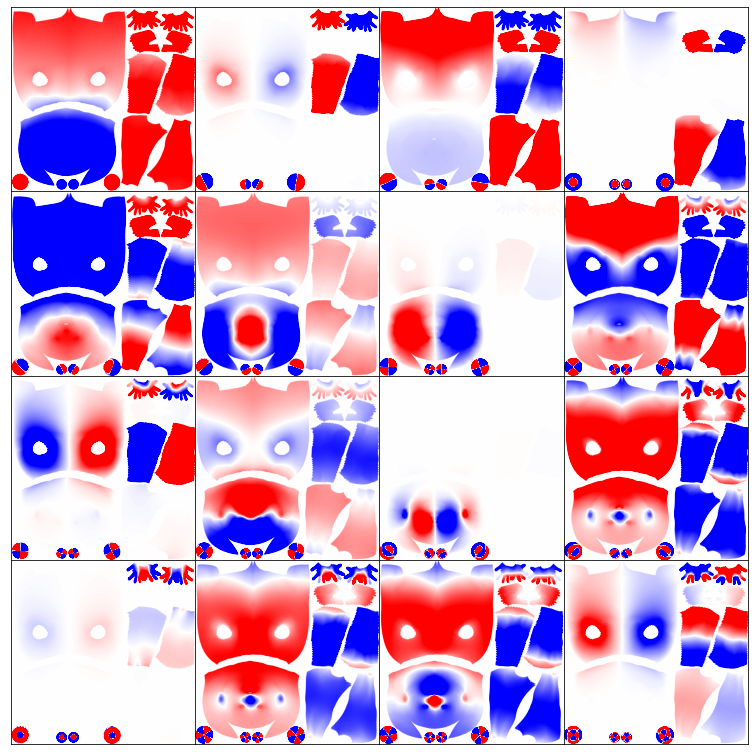
\includegraphics[height=10cm]{\imgfp/other/spectral_ntex}
	\caption{Baseline initialization of a neural texture with $C$ channels, containing $C$ dimensional spectral coordinates of a graph composed of mesh vertices. Notice that in different channels it distinguishes body parts, there is a channel where two legs are colored oppositely, as well as arms, hands, head, upper body, etc. Compared to random initialization, it helps to convey information to the neural renderer about which body part it renders.}
	\label{fig:spectral_ntex}
\end{figure}


\begin{figure}
	\centering
	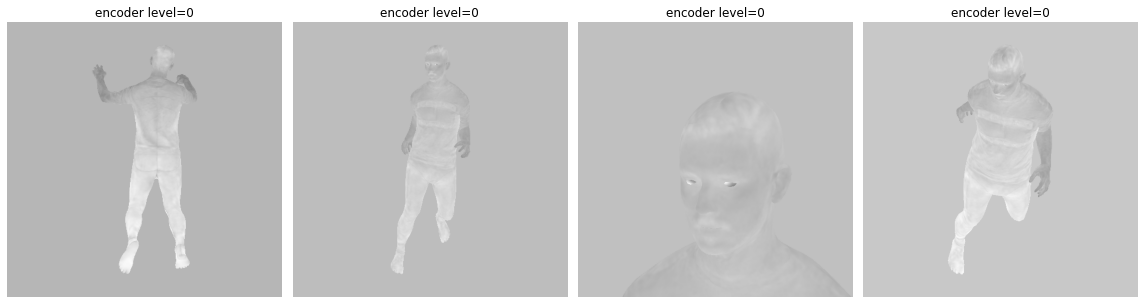
\includegraphics[width=\textwidth]{\imgfp/interm_features/03_e0}%
	\hfill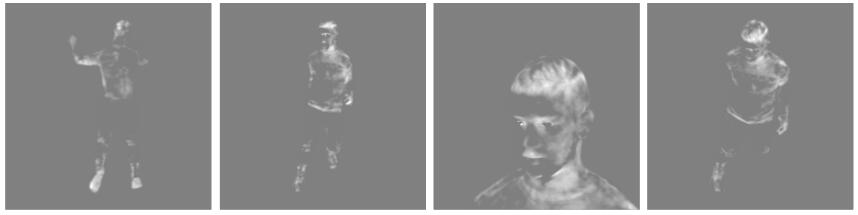
\includegraphics[width=\textwidth]{\imgfp/interm_features/03_e1}%  
	\hfill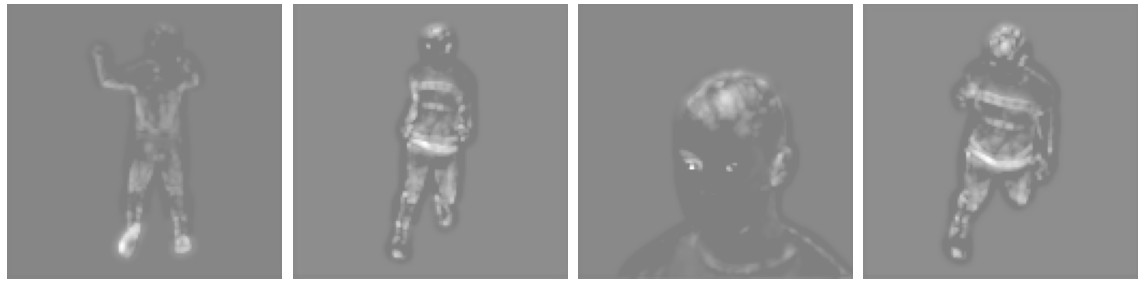
\includegraphics[width=\textwidth]{\imgfp/interm_features/03_e2}%
	\hfill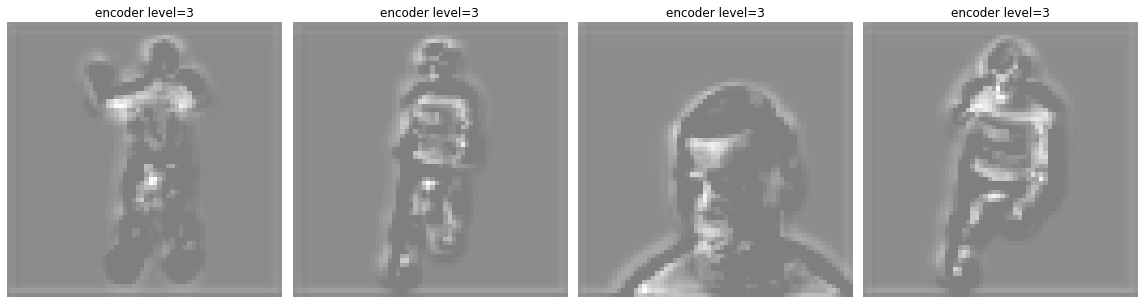
\includegraphics[width=\textwidth]{\imgfp/interm_features/03_e3}%
	\hfill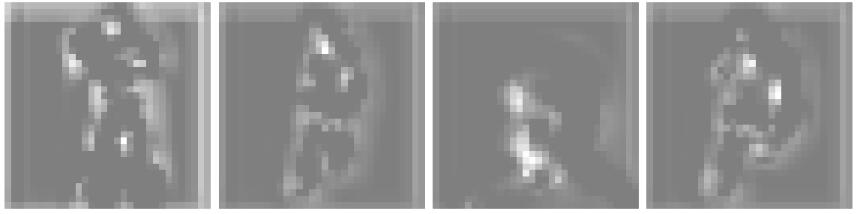
\includegraphics[width=\textwidth]{\imgfp/interm_features/03_e4}%
	\caption{One channel of activations by intermediate levels of the neural renderer's \textit{encoder}. The pipeline is trained on zoomed images. Notice that the features seem activated over the whole body.}
	\label{fig:interm03_encoder}
\end{figure}
\begin{figure}
	\centering
	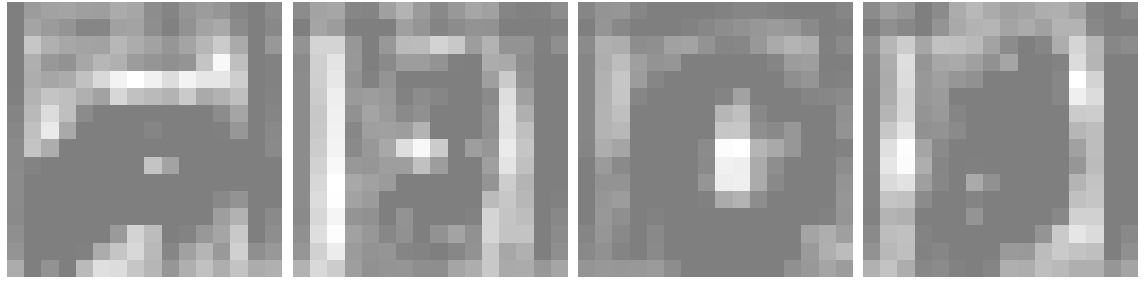
\includegraphics[width=0.9\textwidth]{\imgfp/interm_features/03_d0}%
	\hfill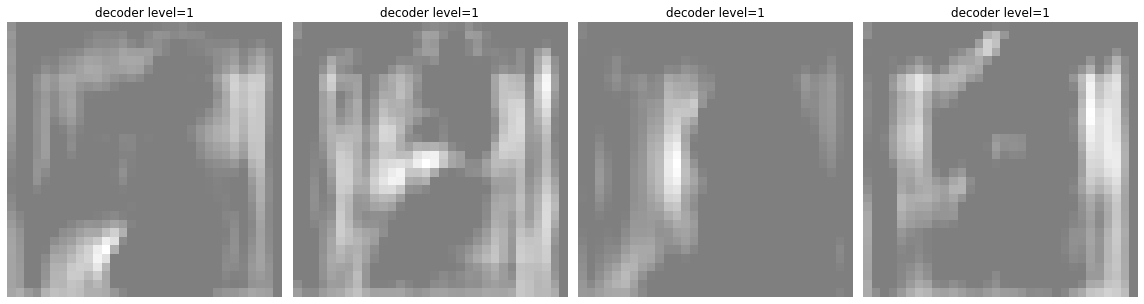
\includegraphics[width=0.9\textwidth]{\imgfp/interm_features/03_d1}%  
	\hfill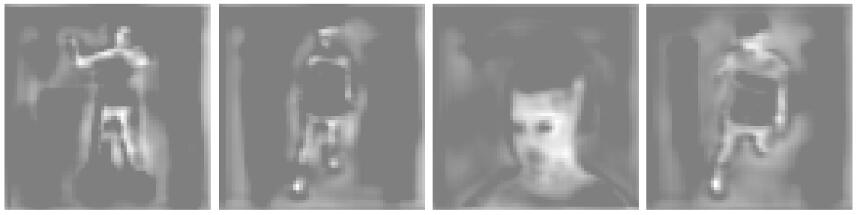
\includegraphics[width=0.9\textwidth]{\imgfp/interm_features/03_d2}%
	\hfill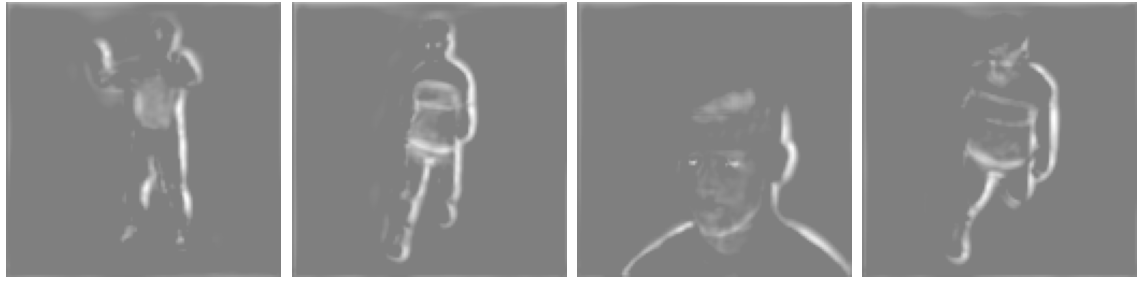
\includegraphics[width=0.9\textwidth]{\imgfp/interm_features/03_d3}%
	\hfill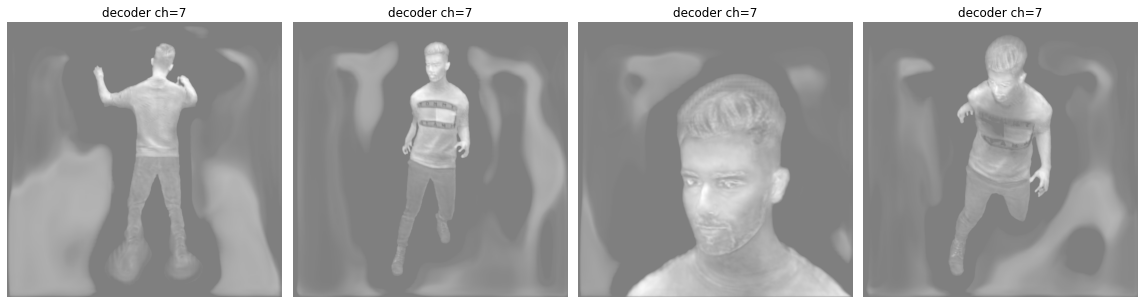
\includegraphics[width=0.9\textwidth]{\imgfp/interm_features/03_dout}%
	\hfill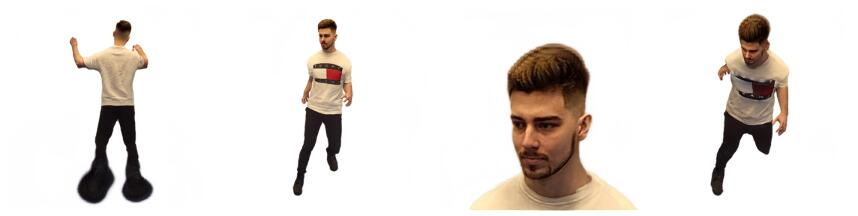
\includegraphics[width=0.9\textwidth]{\imgfp/interm_features/03_rgb}
	\caption{One channel of activations by intermediate levels of the neural renderer's \textit{decoder}. The pipeline is trained on zoomed images. Notice that the space around the human image has a wavy, non-uniform structure. We speculate, that having it helps to make a more accurate segmentation in the neural renderer's heads. }
	\label{fig:interm03_decoder}
\end{figure}
\begin{figure}
	\centering
	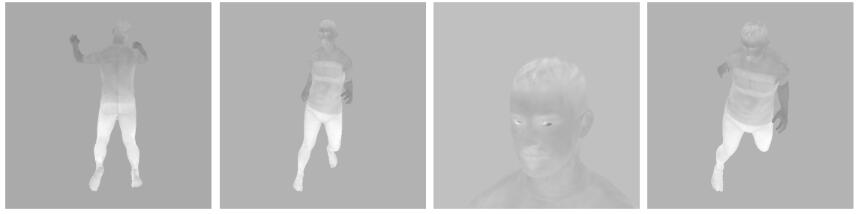
\includegraphics[width=\textwidth]{\imgfp/interm_features/bnf_e0}%
	\hfill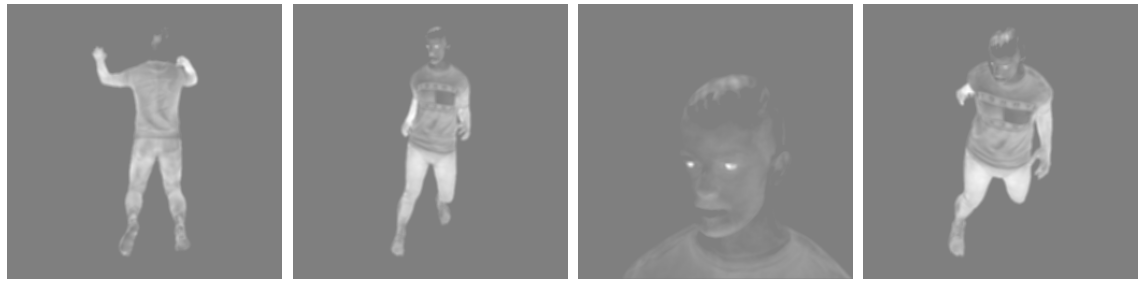
\includegraphics[width=\textwidth]{\imgfp/interm_features/bnf_e1}%  
	\hfill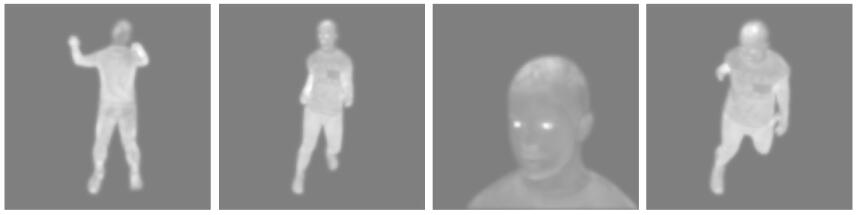
\includegraphics[width=\textwidth]{\imgfp/interm_features/bnf_e2}%
	\hfill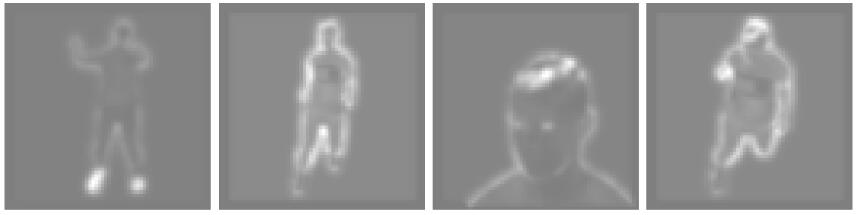
\includegraphics[width=\textwidth]{\imgfp/interm_features/bnf_e3}%
	\hfill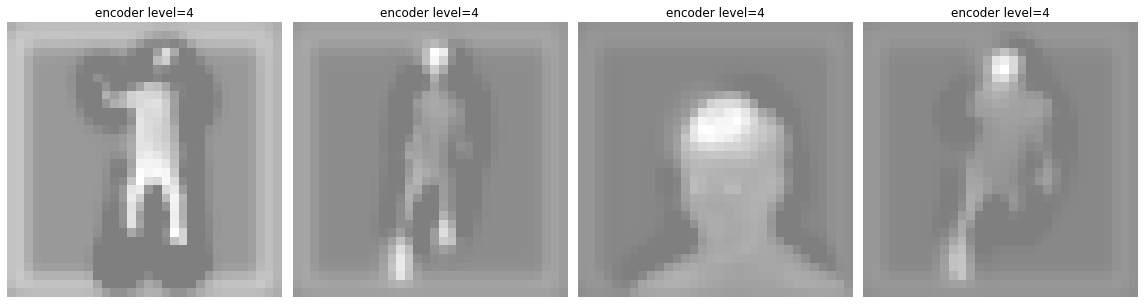
\includegraphics[width=\textwidth]{\imgfp/interm_features/bnf_e4}%
	\caption{One channel of activations by intermediate levels of the neural renderer's \textit{encoder}. The pipeline is trained on zoomed images, but Batch Normalization layers collect running statistics only on full-body images. Notice that some layers specifically trigger on unseen parts of the body that are rarely seen (bottom of boots, top of the head).}
	\label{fig:interm06_encoder}
\end{figure}
\begin{figure}
	\centering
	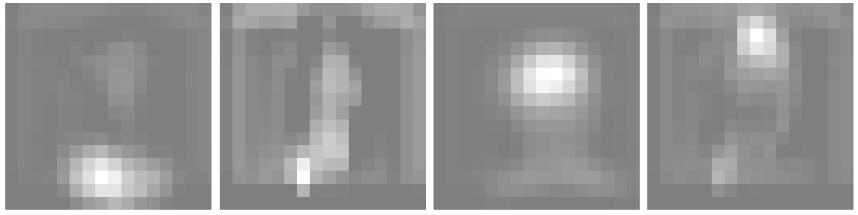
\includegraphics[width=0.9\textwidth]{\imgfp/interm_features/bnf_d0}%
	\hfill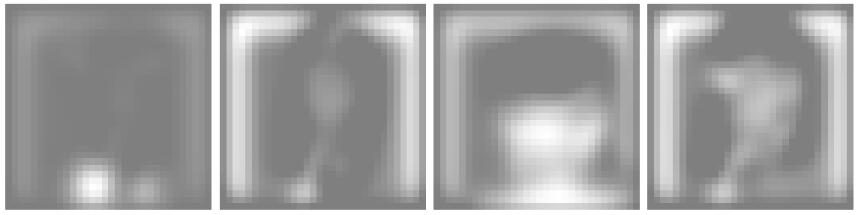
\includegraphics[width=0.9\textwidth]{\imgfp/interm_features/bnf_d1}%  
	\hfill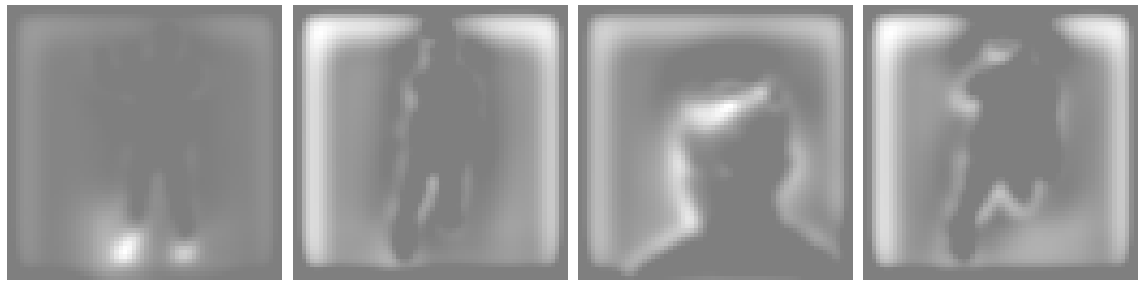
\includegraphics[width=0.9\textwidth]{\imgfp/interm_features/bnf_d2}%
	\hfill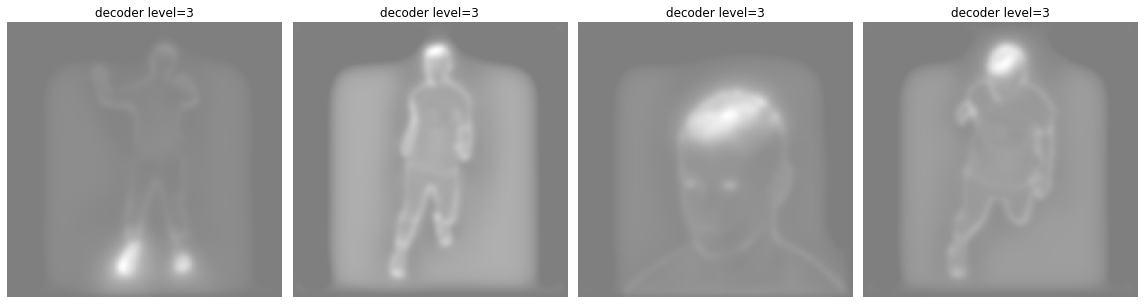
\includegraphics[width=0.9\textwidth]{\imgfp/interm_features/bnf_d3}%
	\hfill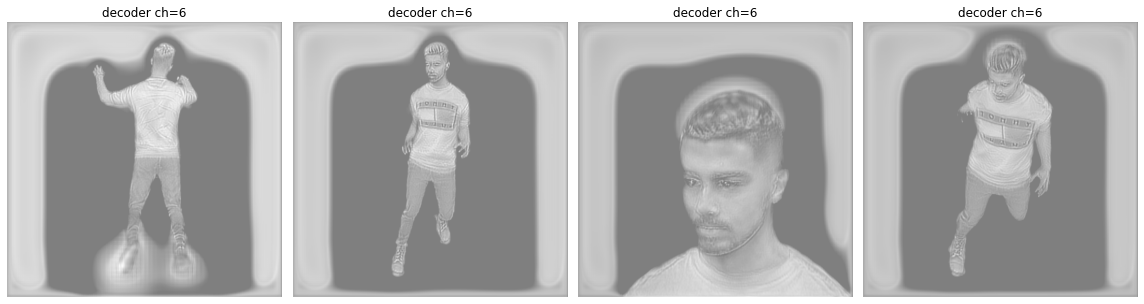
\includegraphics[width=0.9\textwidth]{\imgfp/interm_features/bnf_dout}%
	\hfill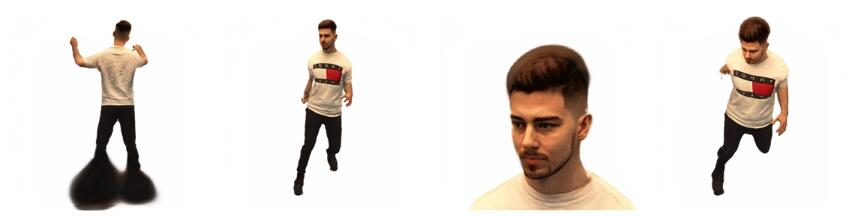
\includegraphics[width=0.9\textwidth]{\imgfp/interm_features/bnf_rgb}%
	\caption{Intermediate activations of the neural renderer's \textit{decoder}, trained on zoomed images, but Batch Normalization layers collect running statistics only on full-body images. Notice that the outer space starts to form a structure that retains one value near the image border, and a sharply different number around the body. We speculate, that this leads to failure in segmentation, and thus the "bubble" effect around the feet and the head. The visual artifacts seem to accumulate as data passes further from the encoder to the decoder. }
	\label{fig:interm06_decoder}
\end{figure}

\begin{figure}
	%\fboxrule=2pt
	\centering
	\begin{subfigure}[b]{0.48\textwidth}
		\centering
		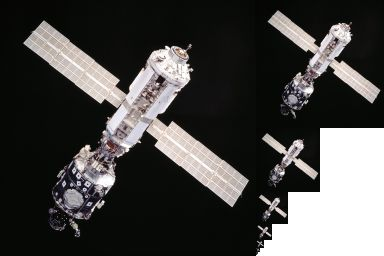
\includegraphics[height=5.5cm]{\imgfp/mips/mipmap}%
		\caption{}
		\label{fig:mipmap}
	\end{subfigure}
	\hfill
	\begin{subfigure}[b]{0.48\textwidth}
		\centering
		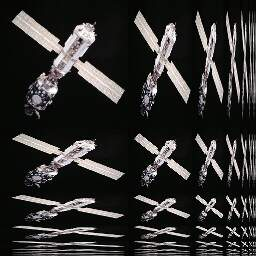
\includegraphics[height=5.5cm]{\imgfp/mips/anisotropic}
		\caption{}
		\label{fig:anisotropic}
	\end{subfigure}
	\caption{(\protect\subref{fig:mipmap}) An example collation of MIP-maps for a texture. It is repeatedly downscaled by a factor of 2, and each scale is pre-processed with an offline filtering algorithm. During rasterization, if a triangle spans a small area on the image, a particular MIP-map scale is chosen to interpolate the texture values. This reduces the aliasing effect (\protect\subref{fig:anisotropic}) Anisotropic filtering pre-processes additional variants for each level of downscales, that are squashed along axes. Images from \href{https://en.wikipedia.org/wiki/Anisotropic_filtering}{en.wikipedia.org/wiki/Anisotropic\_filtering}} 
\end{figure}
\begin{figure}
	\centering
	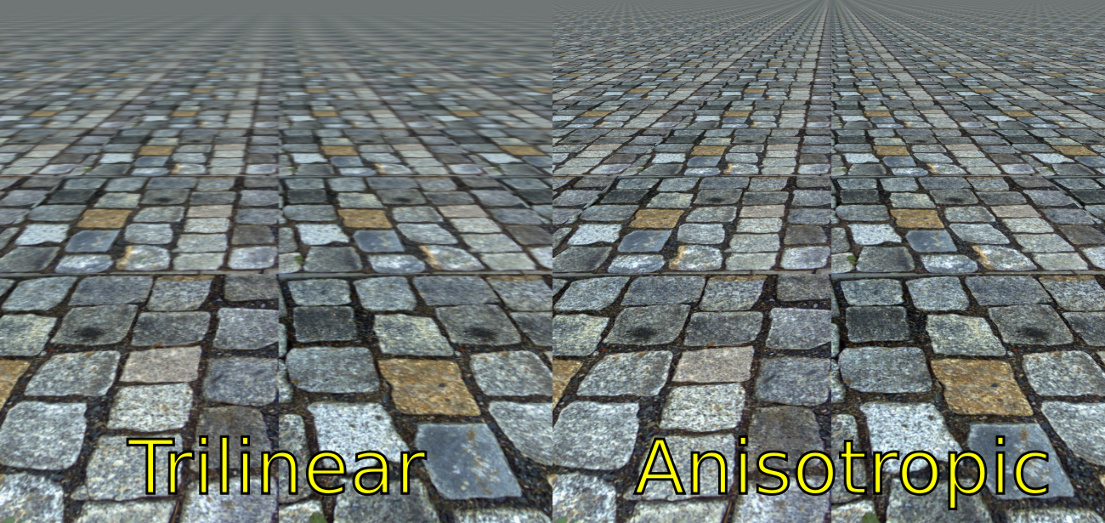
\includegraphics[height=6.5cm]{\imgfp/mips/anisotropic-result-s}
	\caption{By using MIP maps or anisotropically filtered scales of the texture, we could better rasterize triangles that are at steep angles to the camera. Image from \href{https://en.wikipedia.org/wiki/Anisotropic_filtering}{en.wikipedia.org/wiki/Anisotropic\_filtering}}
	\label{fig:anisotropic_result}
\end{figure}
\begin{figure}
	%\fboxrule=2pt
	\centering
	\begin{subfigure}[b]{0.49\textwidth}
		\centering
		\includegraphics[width=\linewidth]{\imgfp/mobile_inference/A01_07_nomips/000435}%
		\caption{}
		\label{fig:no_mipmap_inference}
	\end{subfigure}
	\hfill
	\begin{subfigure}[b]{0.49\textwidth}
		\centering
		\includegraphics[width=\linewidth]{\imgfp/mobile_inference/A01_07_mips_anisotropic/000435}
		\caption{}
		\label{fig:anisotropic_inference}
	\end{subfigure}
	\caption{Comparison of images synthesized on mobile, when MIP mapping with anisotropic filtering is used (\protect\subref{fig:anisotropic_inference}) or not (\protect\subref{fig:no_mipmap_inference}) for rasterization of the input. Unfortunately, the difference is negligible in our case. It can be barely seen on the edges of the mesh, where the triangles face at the most extreme angle to the camera. The processing by the neural renderer further reduces the difference.}
\end{figure}
\begin{figure}
	%\fboxrule=2pt
	\centering
	\begin{subfigure}[b]{0.35\textwidth}
		\centering
		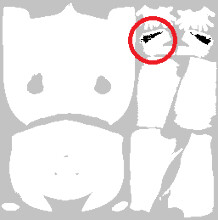
\includegraphics[width=\linewidth]{\imgfp/ntex_patch/ntex-grad}%
		\caption{}
		\label{fig:ntex-grad}
	\end{subfigure}
	\hfill
	\begin{subfigure}[b]{0.3\textwidth}
		\centering
		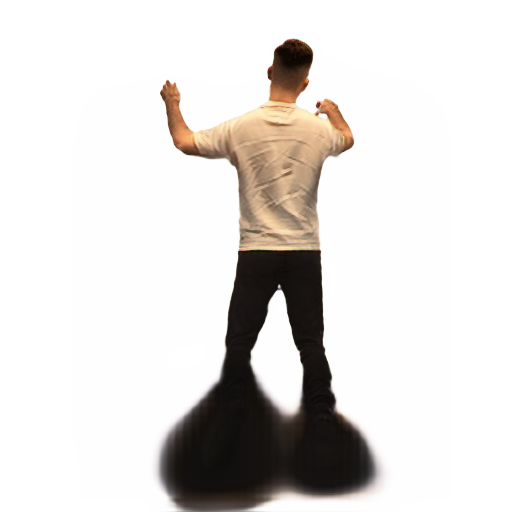
\includegraphics[width=\linewidth]{\imgfp/ntex_patch/fail}
		\caption{}
		\label{fig:ntex-artifact}
	\end{subfigure}
	\hfill
	\begin{subfigure}[b]{0.3\textwidth}
		\centering
		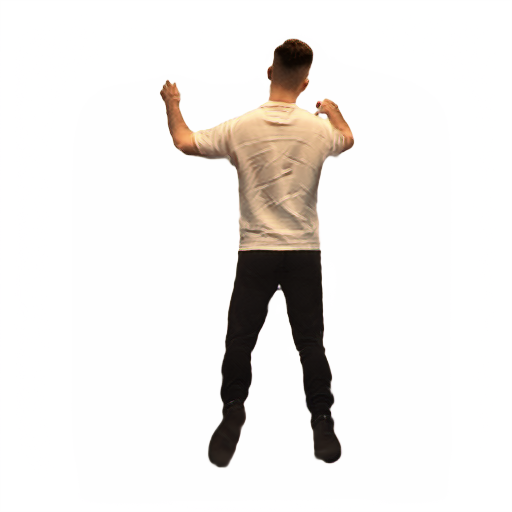
\includegraphics[width=\linewidth]{\imgfp/ntex_patch/fixed}
		\caption{}
		\label{fig:ntex-fixed}
	\end{subfigure}
	\caption{(\protect\subref{fig:ntex-grad}) A mask of non-zero gradients for a neural texture after seeing the whole training sequence. Commonly, some body parts are never seen during training, e.g. bottom of shoes, top of the head, armpits. (\protect\subref{fig:ntex-artifact}) Example of rendering instability due to that. (\protect\subref{fig:ntex-fixed}) A crude solution is to replace the unseen parts with a texture part that was actually optimized (e.g. a part of legs or skin). Although it solves the particular artifact on feet, it may not apply to the head or armpits.}
	\label{fig:ntex-grad-artifact-fixed}
\end{figure}
\begin{figure}
	%\fboxrule=2pt
	\centering
	\begin{subfigure}[b]{0.45\textwidth}
		\centering
		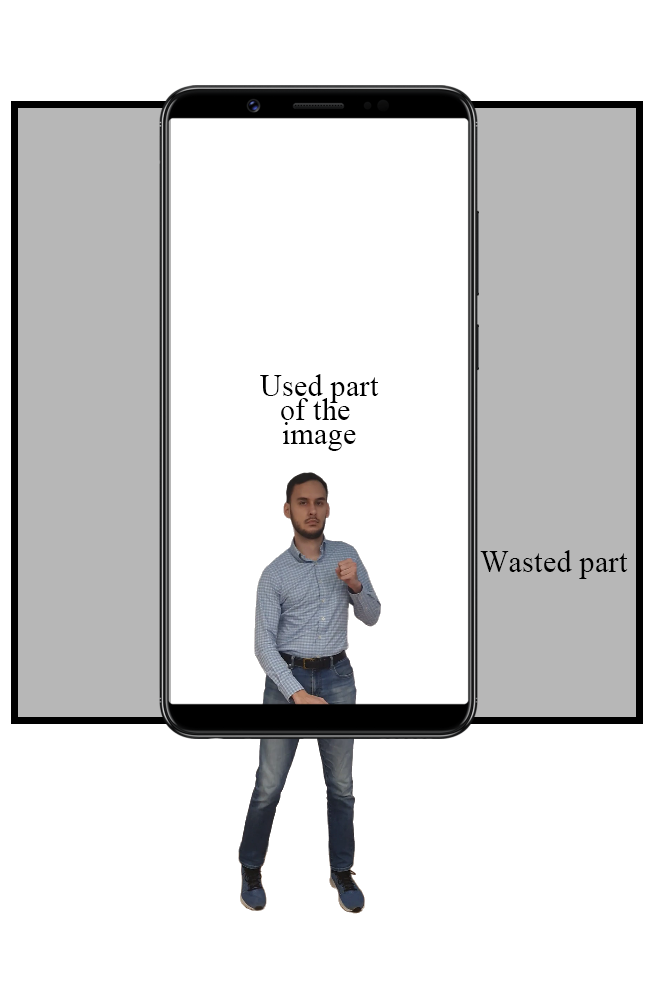
\includegraphics[height=8cm]{\imgfp/dynamic_crop/fullscreen_projection}%
		\caption{}
		\label{fig:explain_crop_fullscreen}
	\end{subfigure}
	\hfill
	\begin{subfigure}[b]{0.27\textwidth}
		\centering
		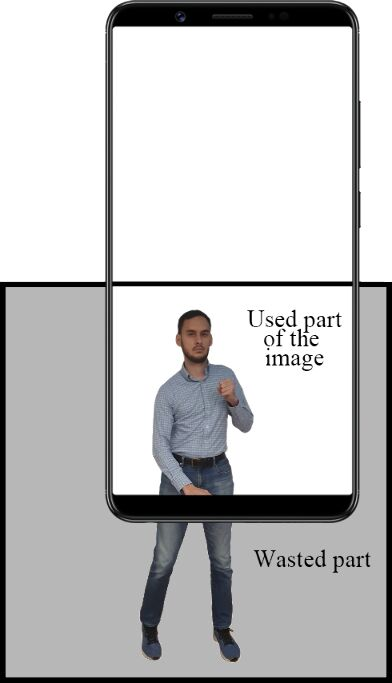
\includegraphics[height=8cm]{\imgfp/dynamic_crop/crop_joints}
		\caption{}
		\label{fig:explain_crop_joints}
	\end{subfigure}
	\hfill
	\begin{subfigure}[b]{0.25\textwidth}
		\centering
		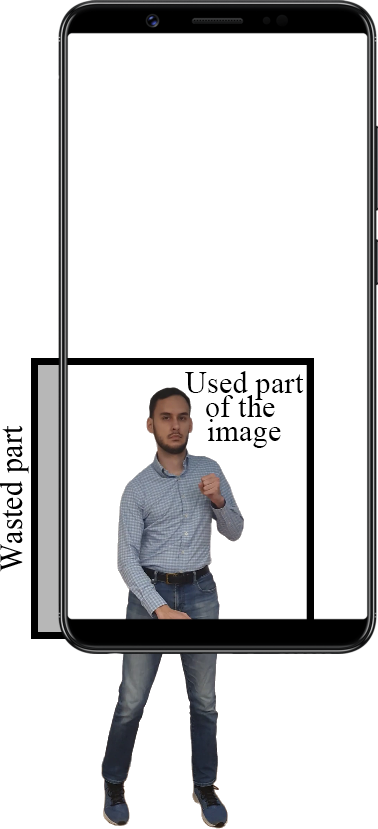
\includegraphics[height=8cm]{\imgfp/dynamic_crop/crop_best}
		\caption{}
		\label{fig:explain_crop_best}
	\end{subfigure}
	\caption{Comparison of projection modes. (\protect\subref{fig:explain_crop_joints}) A projection that spans the whole screen (the default mode). It is additionally widened to make square images (as required for the DNN), and a big part of the generated image is wasted -- time was spent on its computing, but these parts are never shown on the screen. Moreover, the input contains a tiny rasterization of the avatar's body, and unless the neural network was trained to process such small inputs, it may produce visual artifacts (as can be seen in Figure \ref{fig:far_screen_crop}). (\protect\subref{fig:explain_crop_joints}) A dynamic projection crop, that modifies rasterization to always contain the full body in it, regardless of the viewing position. It automatically solves the issues with far-out viewpoints, but still frame parts may be wasted. (\protect\subref{fig:explain_crop_best}) The absolute best dynamic crop that would fit only the part of the body that will be shown on the screen. A fraction of the frame may be wasted to center the body inside the crop. }
	\label{fig:explain_crop}
\end{figure}
\begin{figure}
	\centering%
	\setlength\abovedisplayskip{0pt}%
	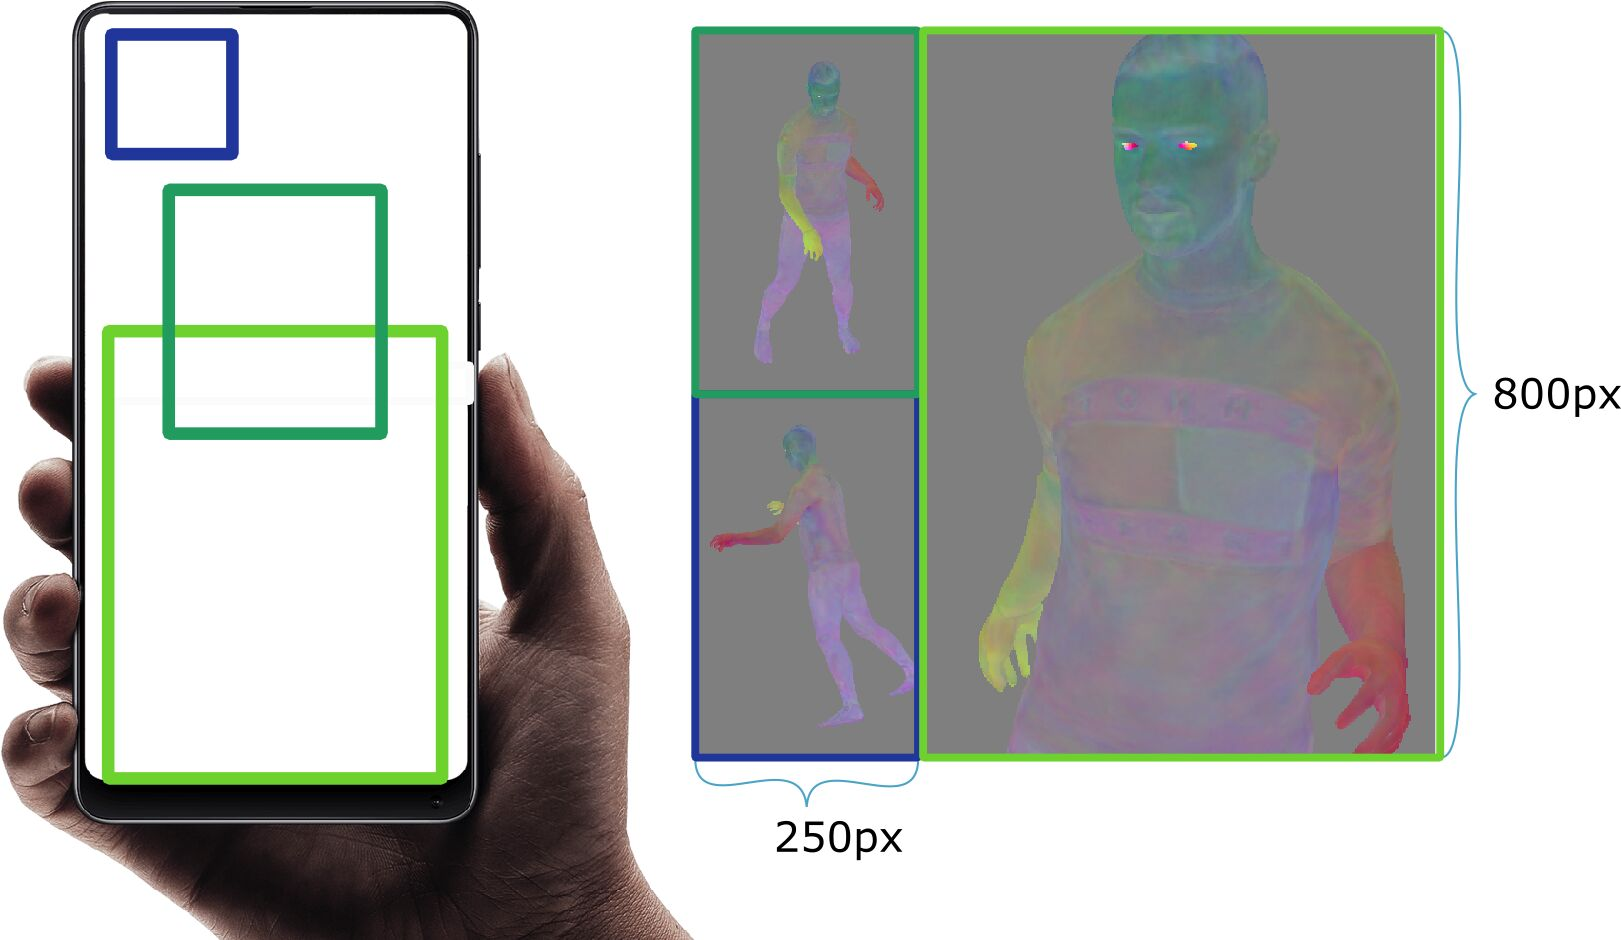
\includegraphics[width=0.6\linewidth]{\imgfp/other/multiavatar}%
	\caption{Example of a future work on inferring images of multiple avatars. Inputs can be dynamically cropped, rasterized at a resolution proportional to occupied space, and collated into a single input tensor. Knowing the screen location of the avatars, the synthesized images can be rendered at proper locations in AR.}%
	\label{fig:multiavatar}%
	\setlength\belowdisplayskip{0pt}%
\end{figure}
%\setkeys{Gin}{draft=false}
\begin{figure}
	\centering
	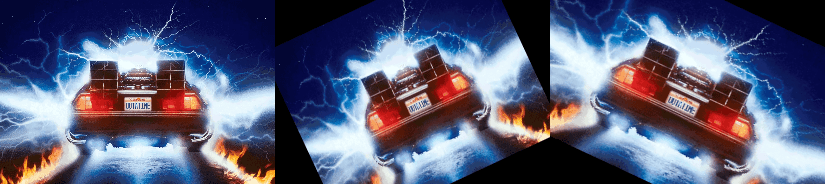
\includegraphics[width=\textwidth]{\imgfp/other/warp_affine}
	\caption{An example of image-space affine augmentations that can be applied to an image. They perform 2D rotation, scale, and translation. Since after the rotation the image may not align with the pixel grid, the specific pixel values are calculated as a bilinear interpolation between old transformed pixels. The image from \href{https://kornia.readthedocs.io/en/latest/geometry.transform.html}{https://kornia.readthedocs.io/en/latest/geometry.transform.html}.}
	\label{fig:image-space-aug-kornia}
\end{figure}

\begin{figure}
	\centering
	\begin{subfigure}[b]{0.49\textwidth}
		\centering
		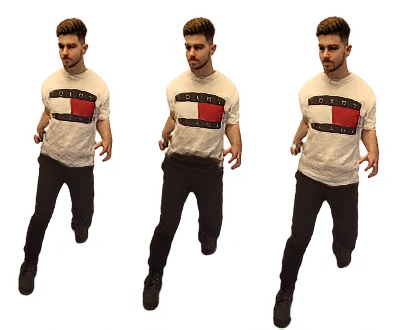
\includegraphics[height=7cm]{\imgfp/spurious/zoom-spurious}
		\caption{}
		\label{fig:spurious_zoom}
	\end{subfigure}
	\hfill
	\begin{subfigure}[b]{0.49\textwidth}
		\centering
		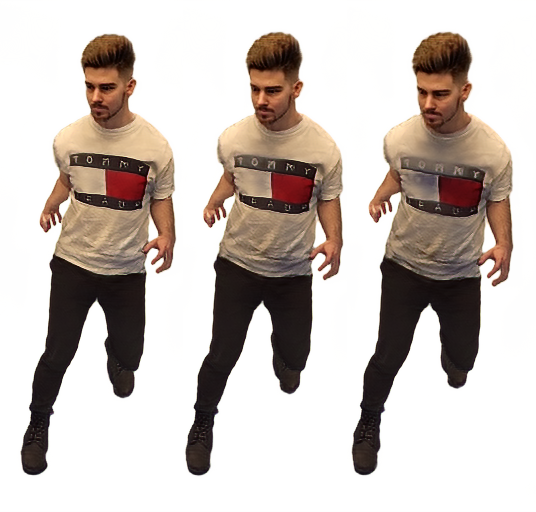
\includegraphics[height=7cm]{\imgfp/spurious/rotation-spurious}
		\caption{}
		\label{fig:spurious_rotation}
	\end{subfigure}
	\caption{Examples of a visual artifact, connected to DNN overfitting, which we refer to as \textit{spurious correlations}. Frames with similar poses or camera views may be rendered with occasional drastic changes. It may appear as a change of creases on the clothes, warping of clothes, or a change of lighting all over the avatar. (\protect\subref{fig:spurious_zoom}) A tiny change of scale (zooming in) leads to instability. (\protect\subref{fig:spurious_rotation}) A tiny change of rotation towards top-down leads to instability. See Figure \ref{fig:overfitting_gt} with problematic ground truth images that trigger this effect of a "shade" on the avatar.}
	\label{fig:spurious}
\end{figure}

\begin{figure}
	\centering
	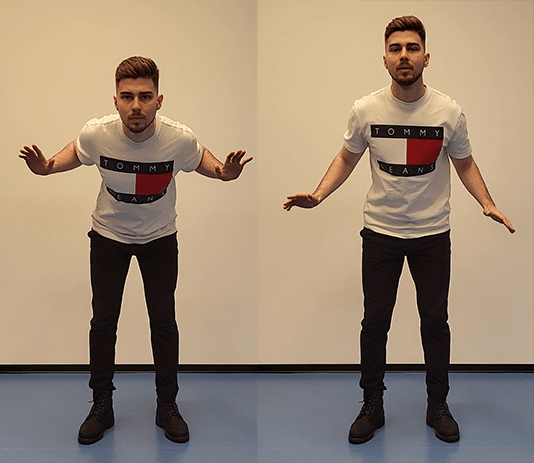
\includegraphics[height=9cm]{\imgfp/spurious/gt-min}
	\caption{Two not-so-distant frames from the ground truth video sequence, however, they have a great difference in color on the T-shirt due to different light conditions. If the rendering DNN overfits the training data, the synthesized images may be unstable and contain such drastic flickering of color. }
	\label{fig:overfitting_gt}
\end{figure}

%\setkeys{Gin}{draft}
\section{Mobile application}
\label{appb:mobile-screenshots}

\begin{figure}[h]
	%\fboxrule=2pt
	\centering
	\begin{subfigure}[b]{0.32\textwidth}
		\centering
		\includegraphics[width=\linewidth]{\imgfp/mobile_inference/A01_07_gpu/000435}%
		\caption{}
		\label{fig:infer_gpu}
	\end{subfigure}
	\hfill
	\begin{subfigure}[b]{0.32\textwidth}
		\centering
		\includegraphics[width=\linewidth]{\imgfp/mobile_inference/A01_07_dsp/000435}
		\caption{}
		\label{fig:infer_dsp}
	\end{subfigure}
	\hfill
	\begin{subfigure}[b]{0.32\textwidth}
		\centering
		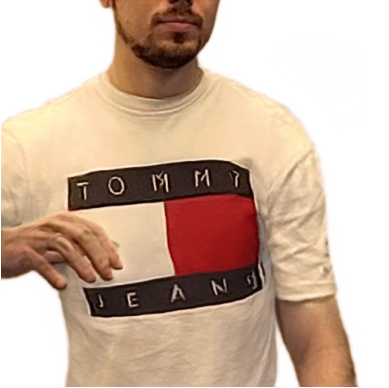
\includegraphics[width=\linewidth]{\imgfp/mobile_inference/A01_07_desktop/mobile_on_desktop35w}
		\caption{}
		\label{fig:infer_desktop}
	\end{subfigure}
	\caption{Comparison of quality loss when synthesizing images on a mobile phone or desktop computer. (\protect\subref{fig:infer_gpu}) was generated on mobile GPU from INT8 quantized input and FP32 weights. (\protect\subref{fig:infer_dsp}) was synthesized on mobile DSP with both input and weights quantized to INT8. It has noticeable discretization noise. (\protect\subref{fig:infer_desktop}) was generated on a desktop GPU using PyTorch with initial FP32 inputs and network weights. The quality is identical to the mobile GPU.}
	\label{fig:infer_different_devices}
\end{figure}
\begin{figure}[hb]
	%\fboxrule=2pt
	\centering
	\begin{subfigure}[b]{0.3\textwidth}
		\centering
		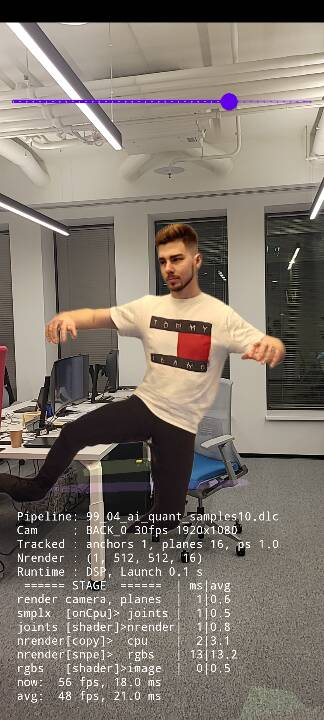
\includegraphics[width=\linewidth]{\imgfp/mobile_screenshots/jump}%
		\caption{}
		\label{fig:mobile_example_jump}
	\end{subfigure}
	\hfill
	\begin{subfigure}[b]{0.3\textwidth}
		\centering
		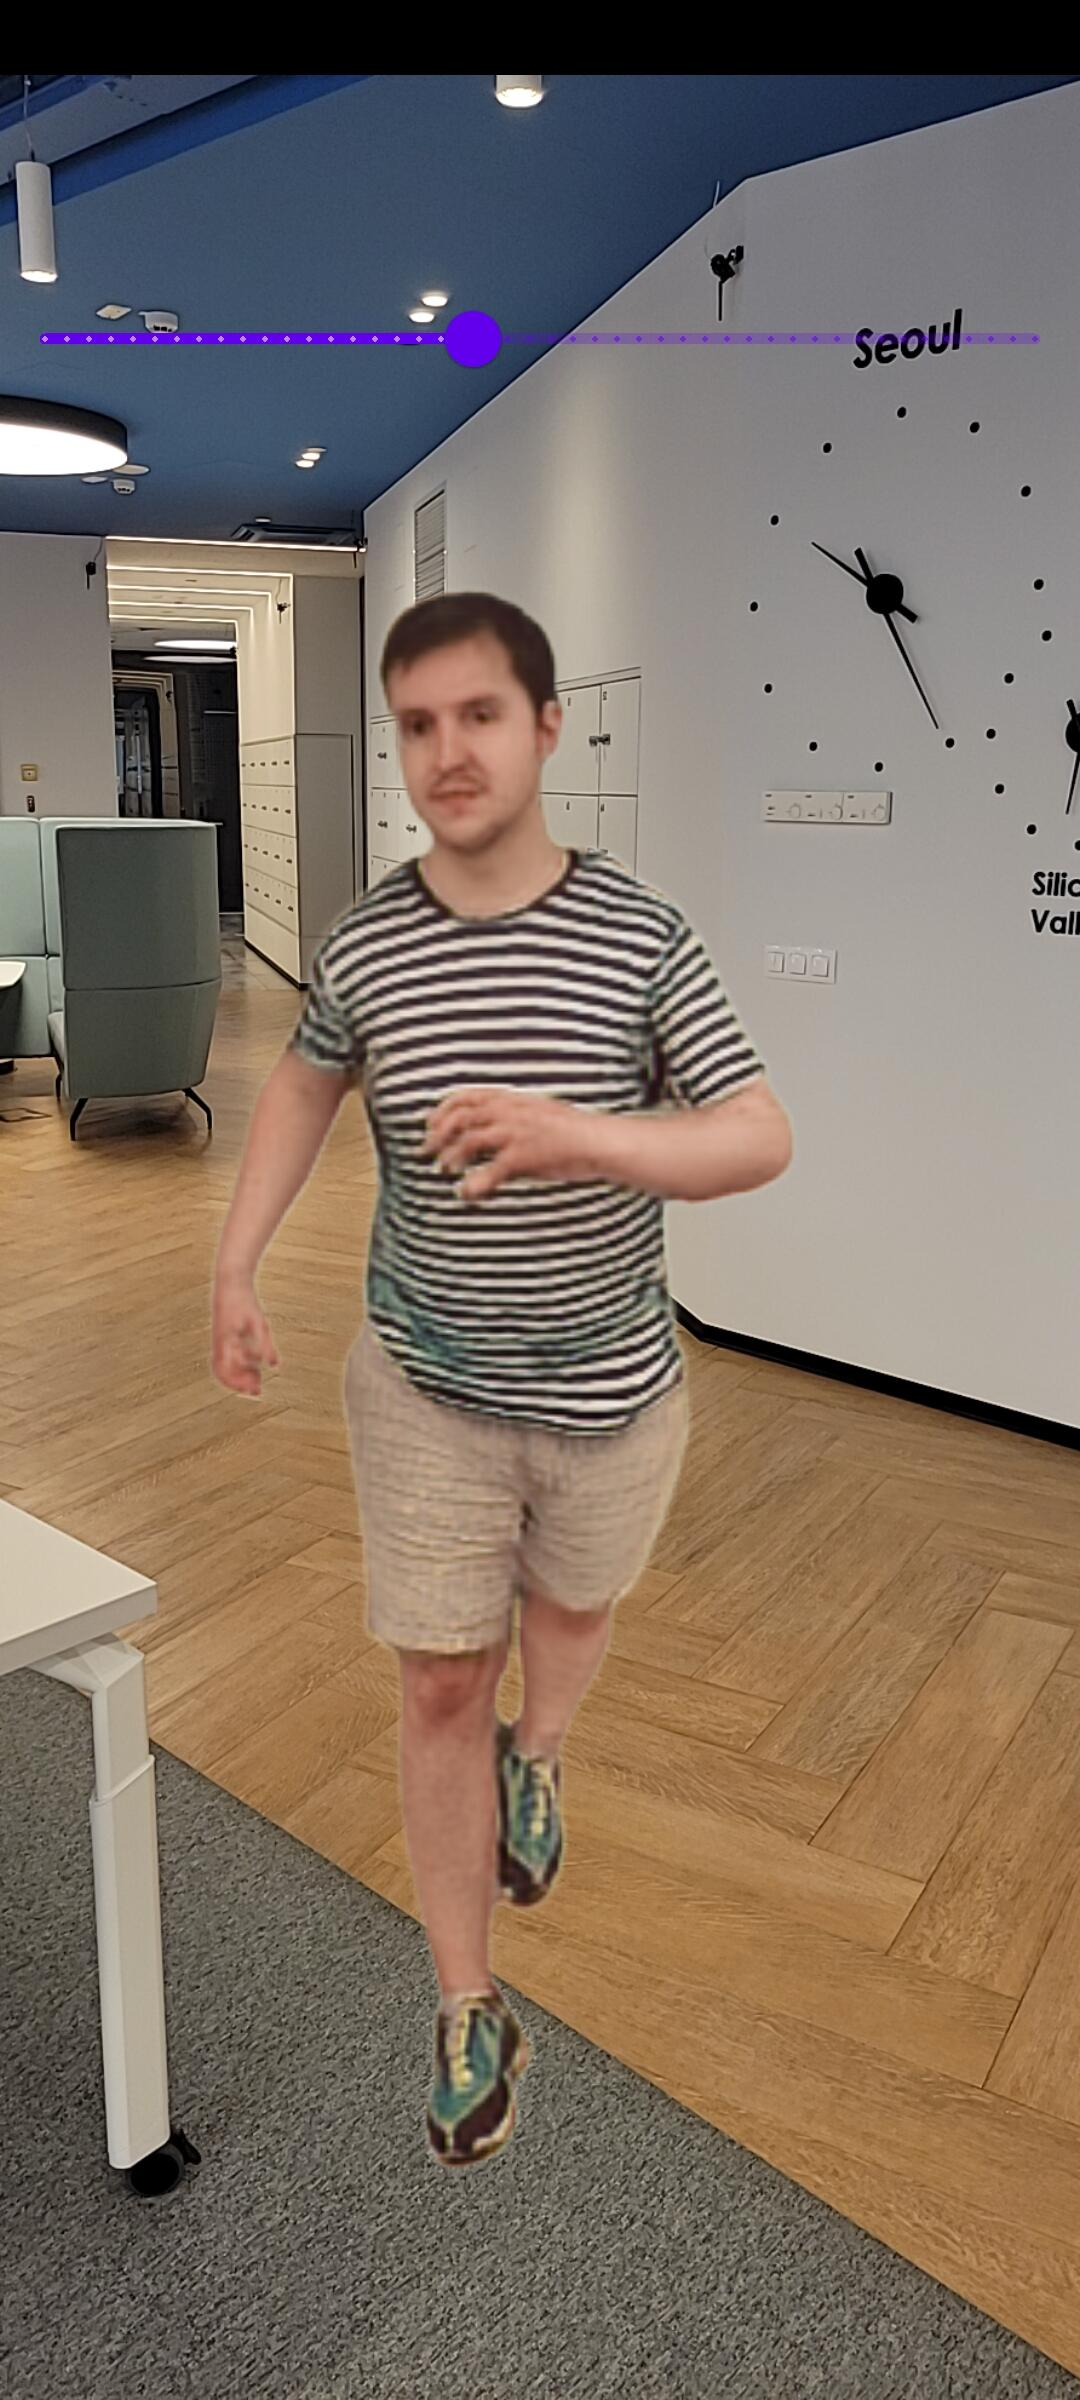
\includegraphics[width=\linewidth]{\imgfp/mobile_screenshots/example_egor}
		\caption{}
	\end{subfigure}
	\hfill
	\begin{subfigure}[b]{0.3\textwidth}
		\centering
		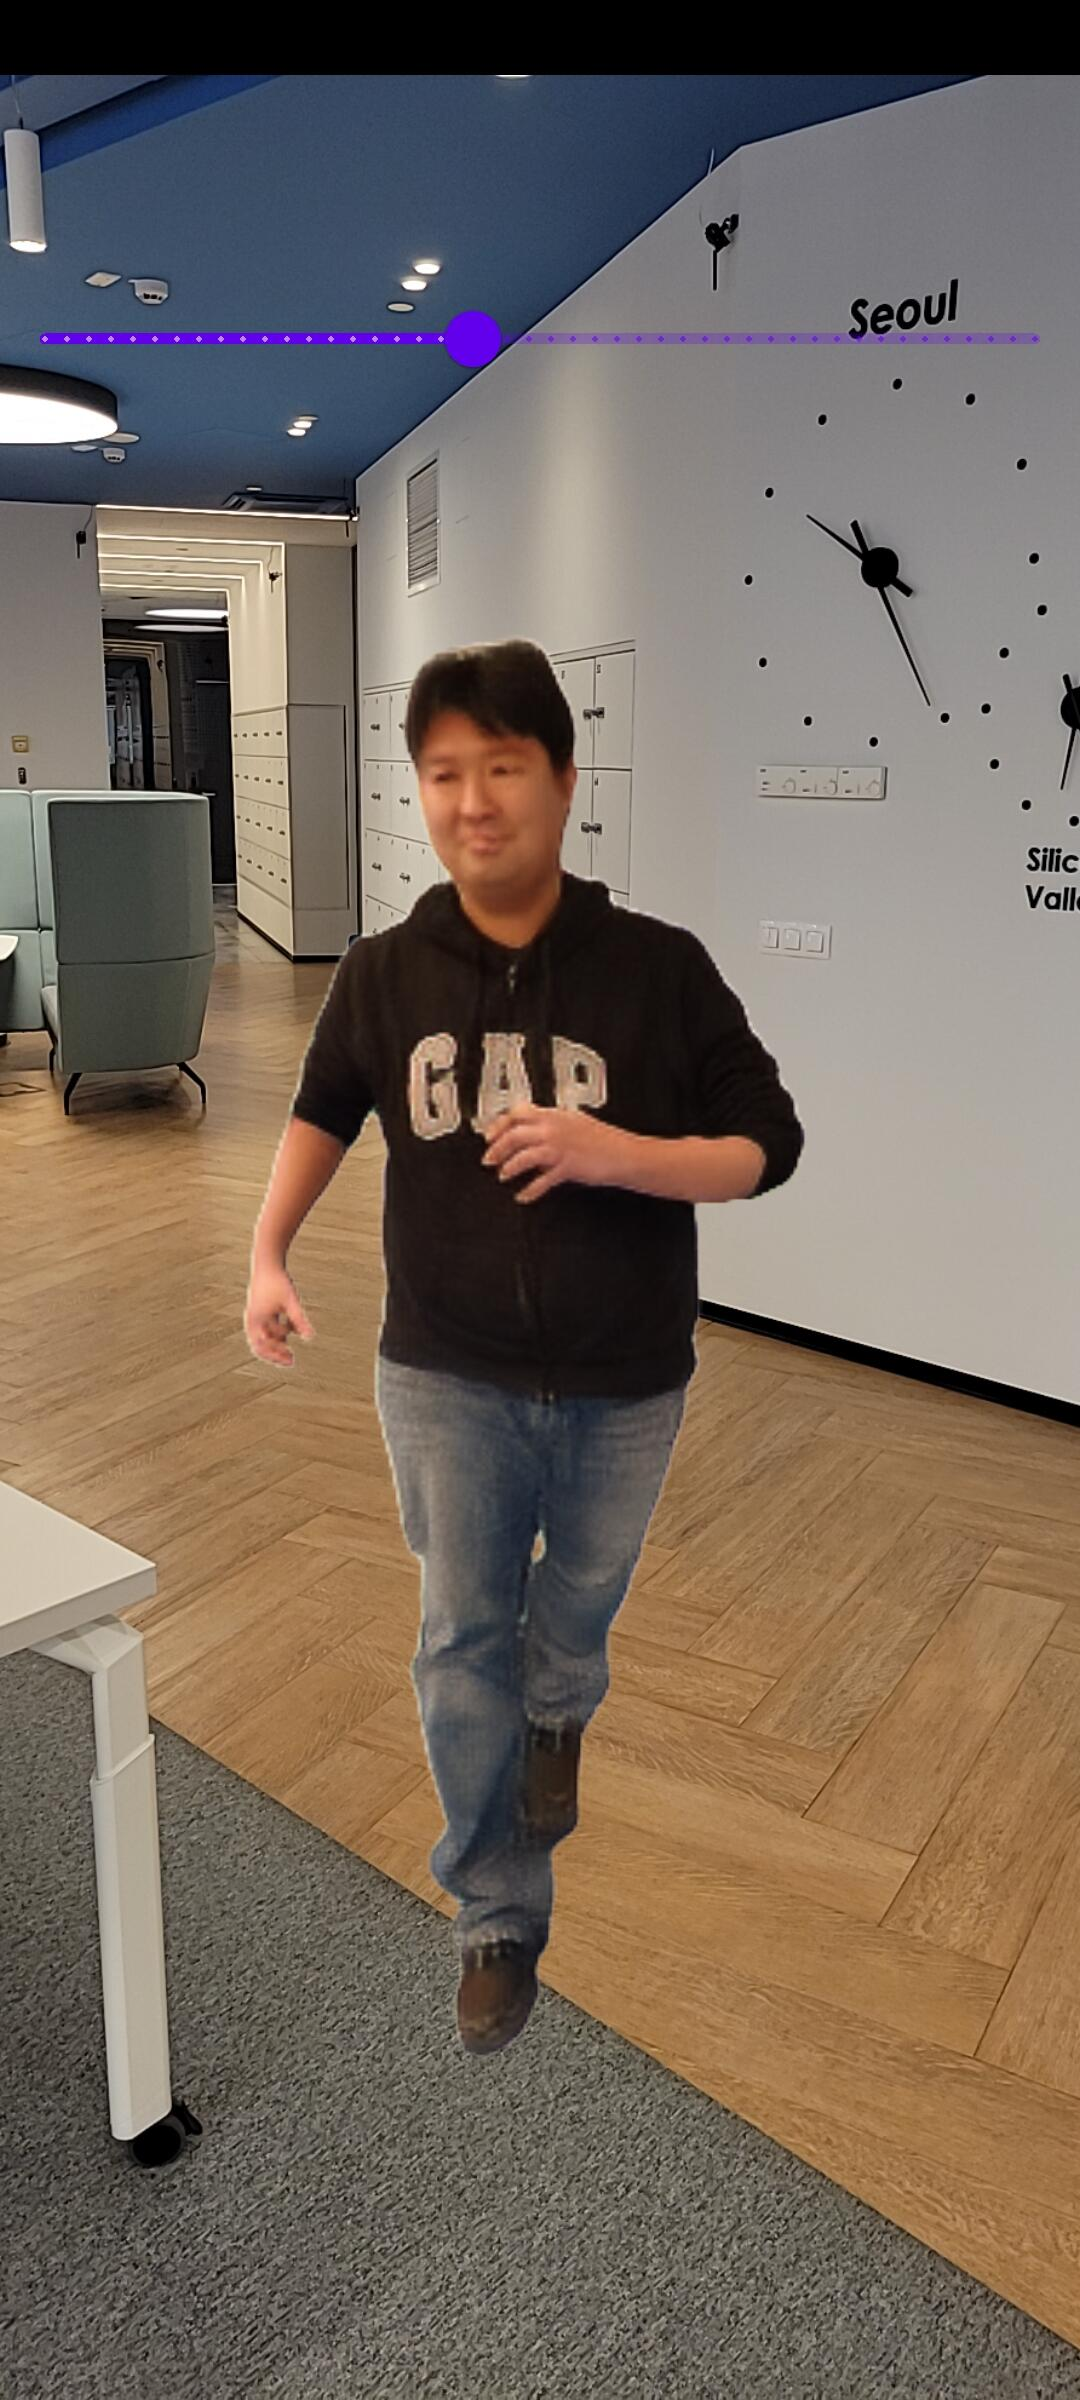
\includegraphics[width=\linewidth]{\imgfp/mobile_screenshots/example_minsoo}
		\caption{}
	\end{subfigure}
	\vspace{1em}
		\begin{subfigure}[b]{0.3\textwidth}
		\centering
		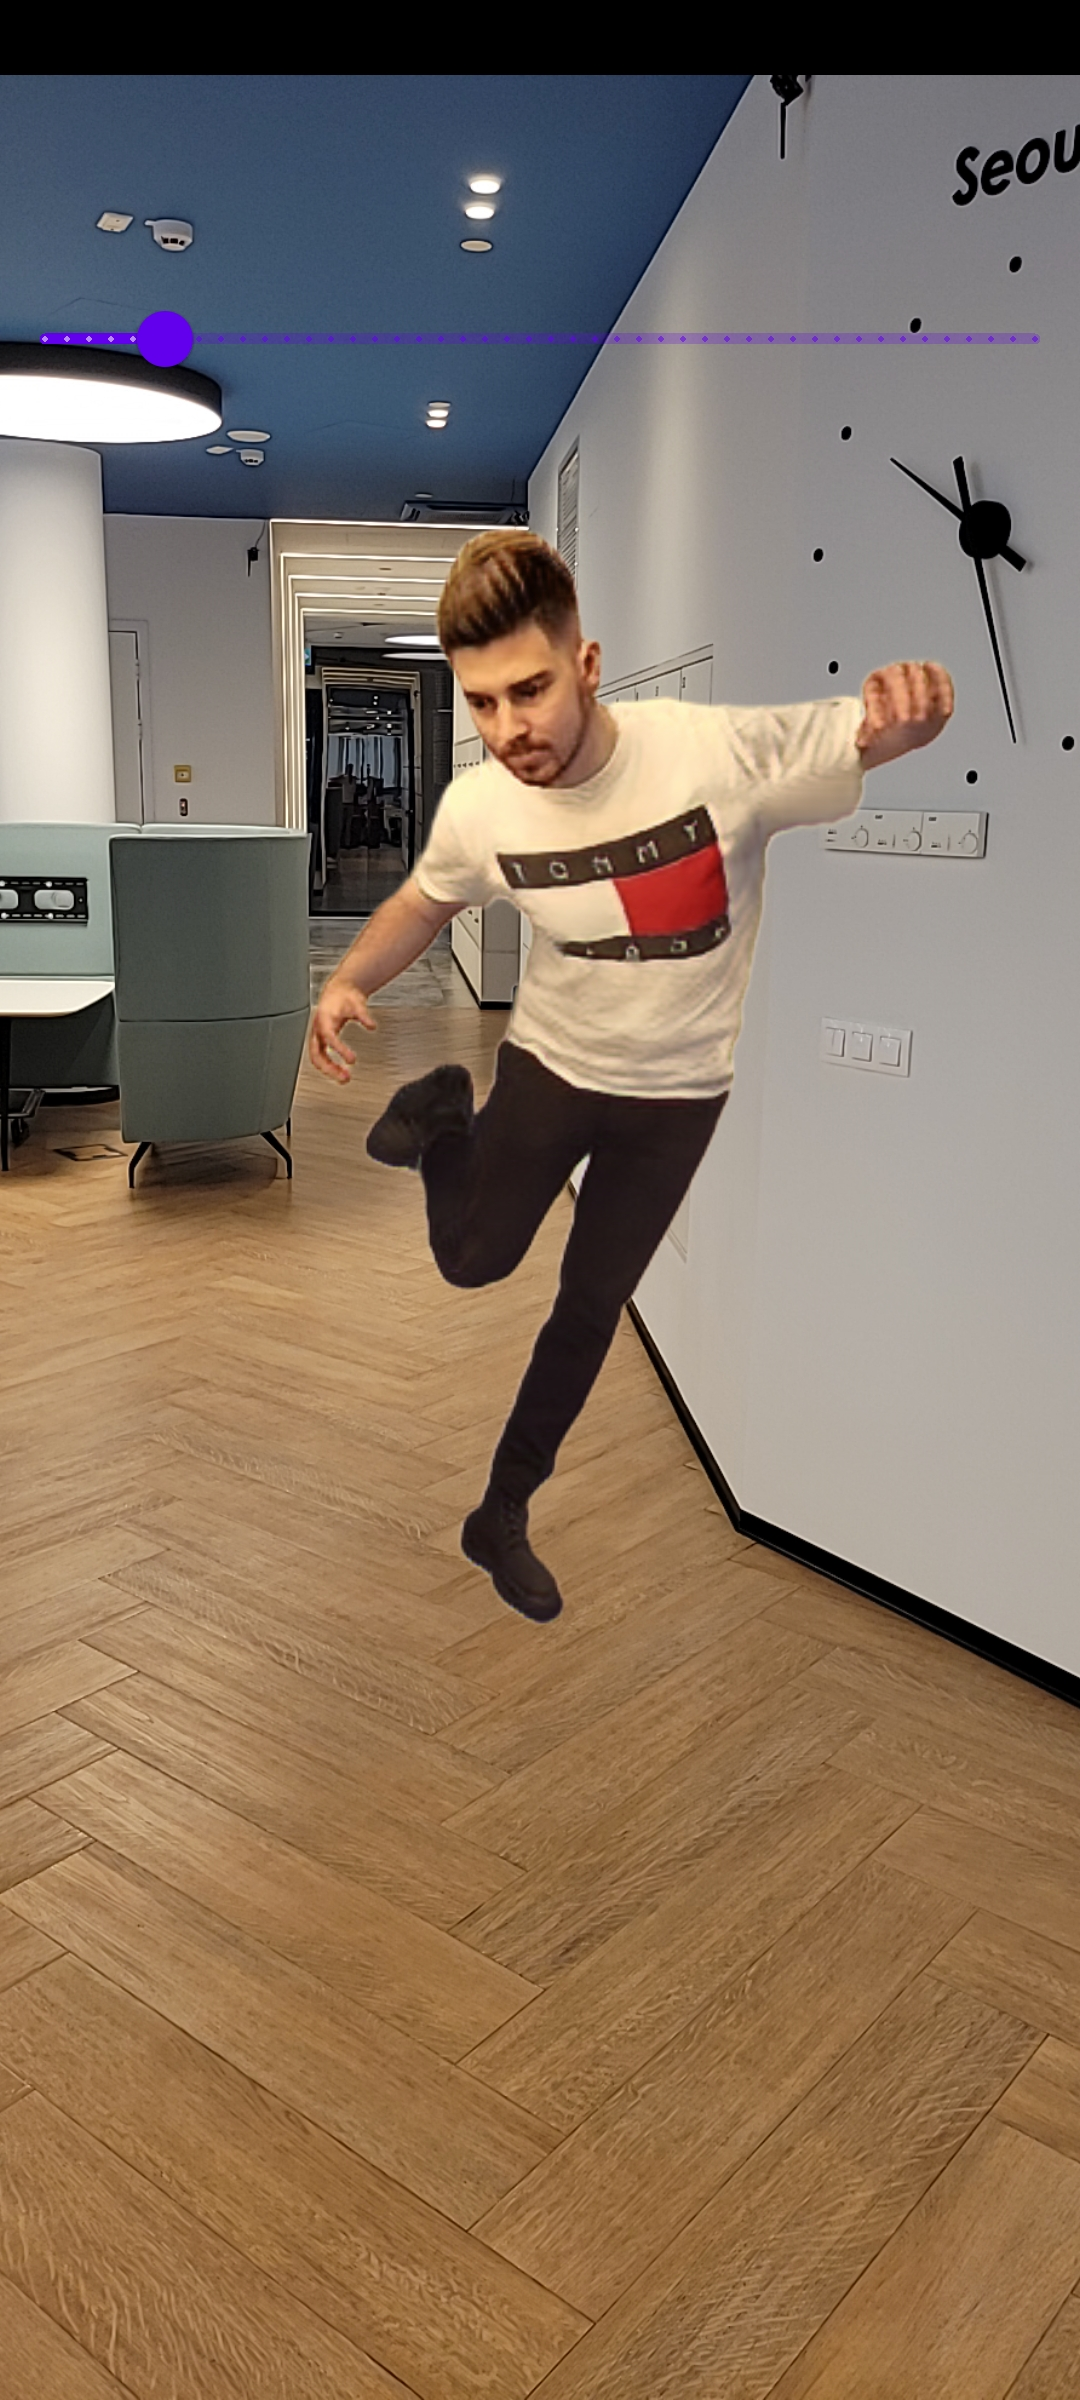
\includegraphics[width=\linewidth]{\imgfp/mobile_screenshots/example_ilya}%
		\caption{}
	\end{subfigure}
	\hfill
	\begin{subfigure}[b]{0.3\textwidth}
		\centering
		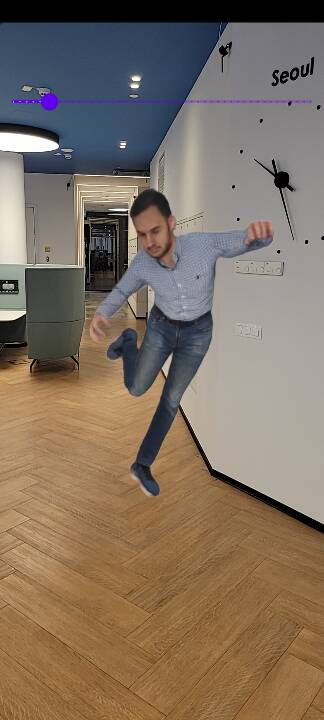
\includegraphics[width=\linewidth]{\imgfp/mobile_screenshots/example_renat}
		\caption{}
		\label{fig:mobile_example_renat}
	\end{subfigure}
	\hfill
	\begin{subfigure}[b]{0.3\textwidth}
		\centering
		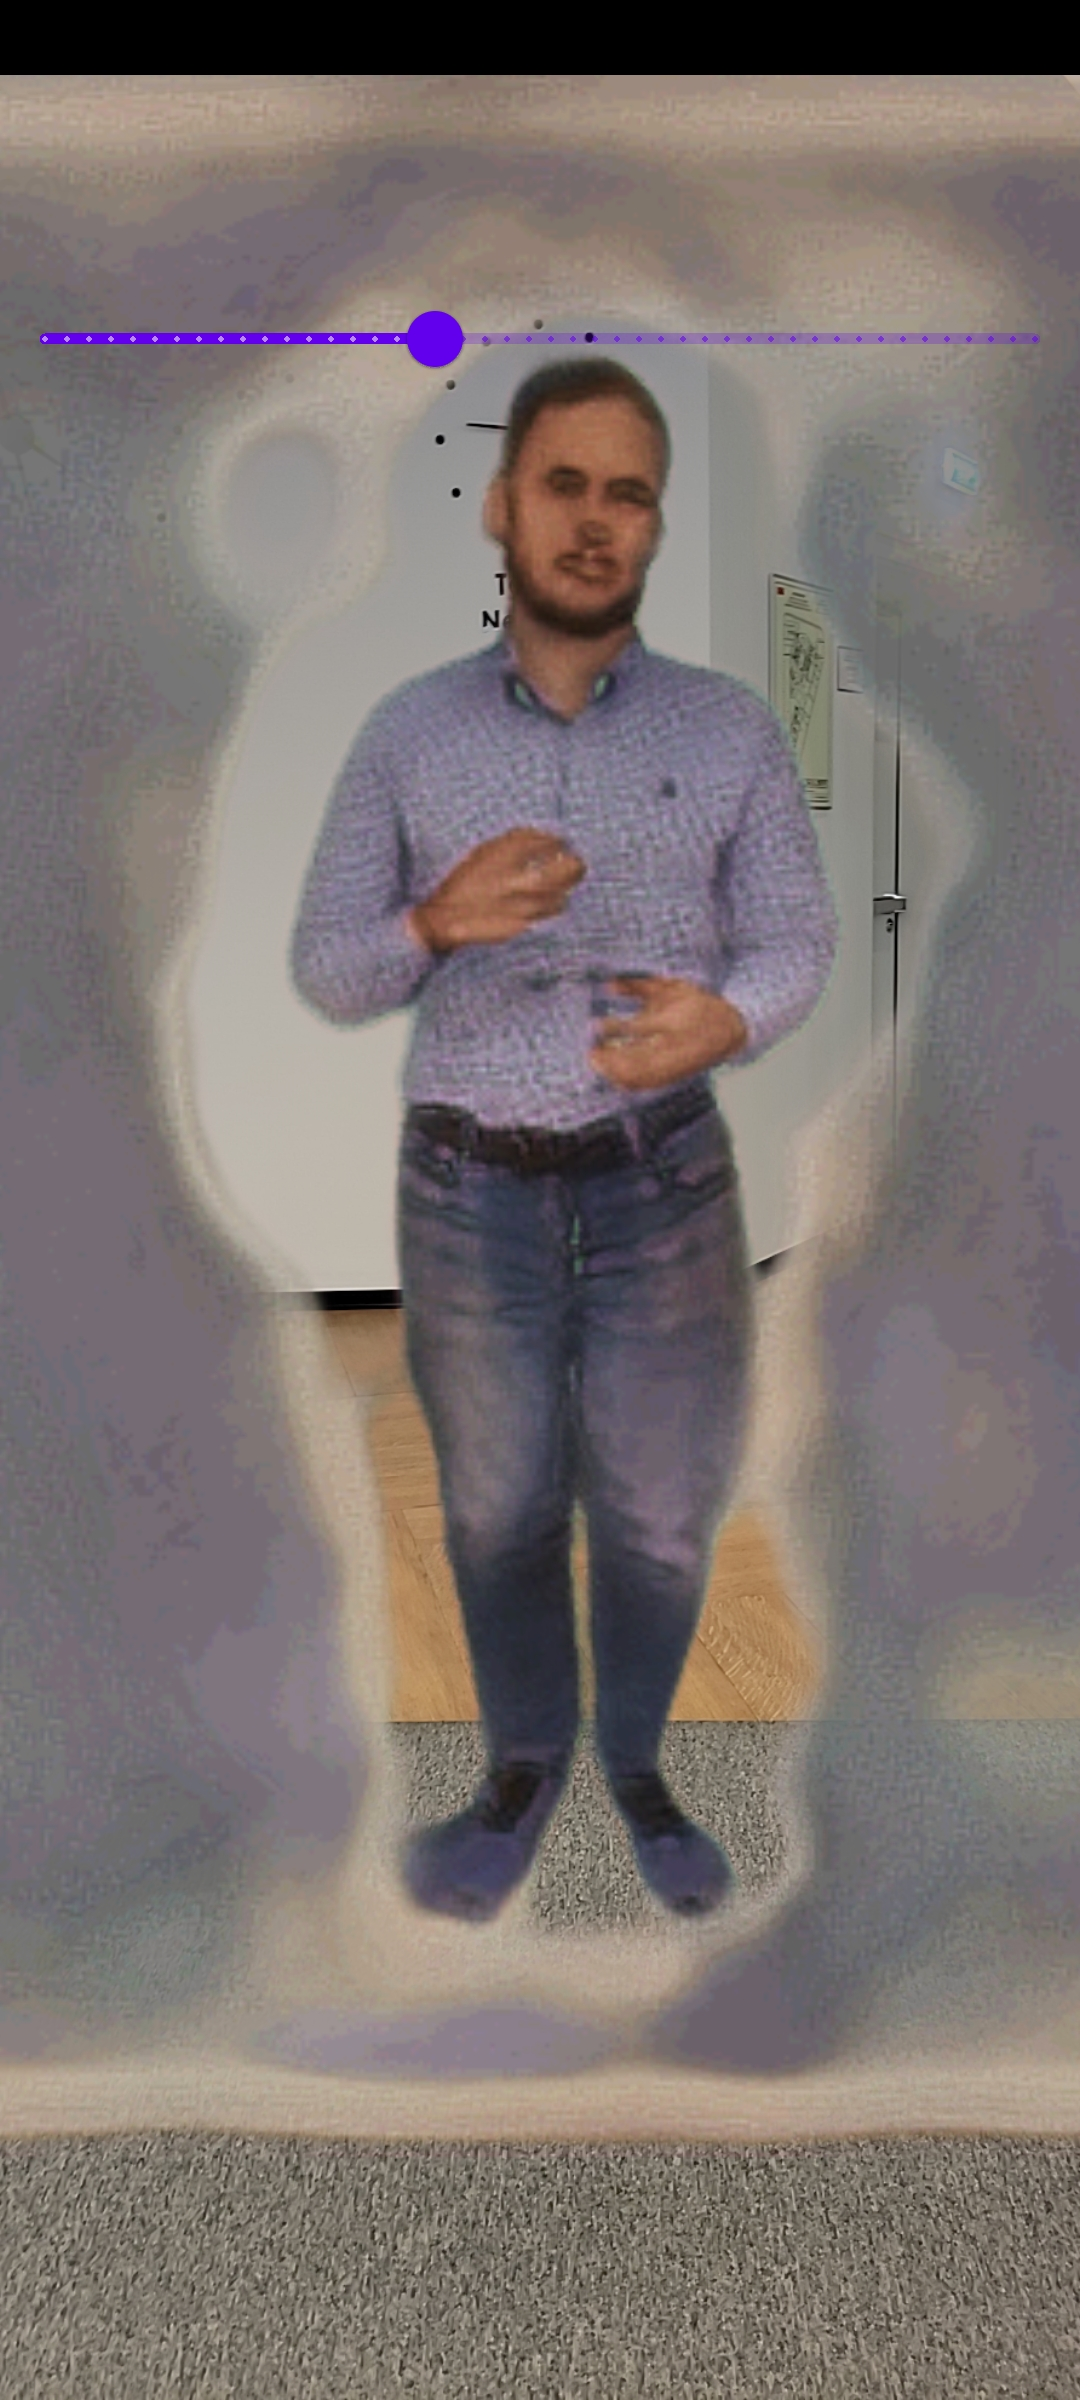
\includegraphics[width=\linewidth]{\imgfp/mobile_screenshots/tf_effnet_dsp}
		\caption{}
		\label{fig:mobile_tf_effent_fail}
	\end{subfigure}
	\caption{(\protect\subref{fig:mobile_example_jump}-\protect\subref{fig:mobile_example_renat}) Examples of avatar images in the mobile application. We have predefined animations that can be played with any avatar. (\protect\subref{fig:mobile_tf_effent_fail}) A case of using another backbone for the renderer (EfficientNet \cite{dnn:efficientnetv1-19}), it has worse quality after training, moreover, on the mobile DSP it fails to synthesize correct segmentation. }
	\label{fig:mobile_example}
\end{figure}
\begin{figure}
	%\fboxrule=2pt
	\centering
	\begin{subfigure}[b]{0.32\textwidth}
		\centering
		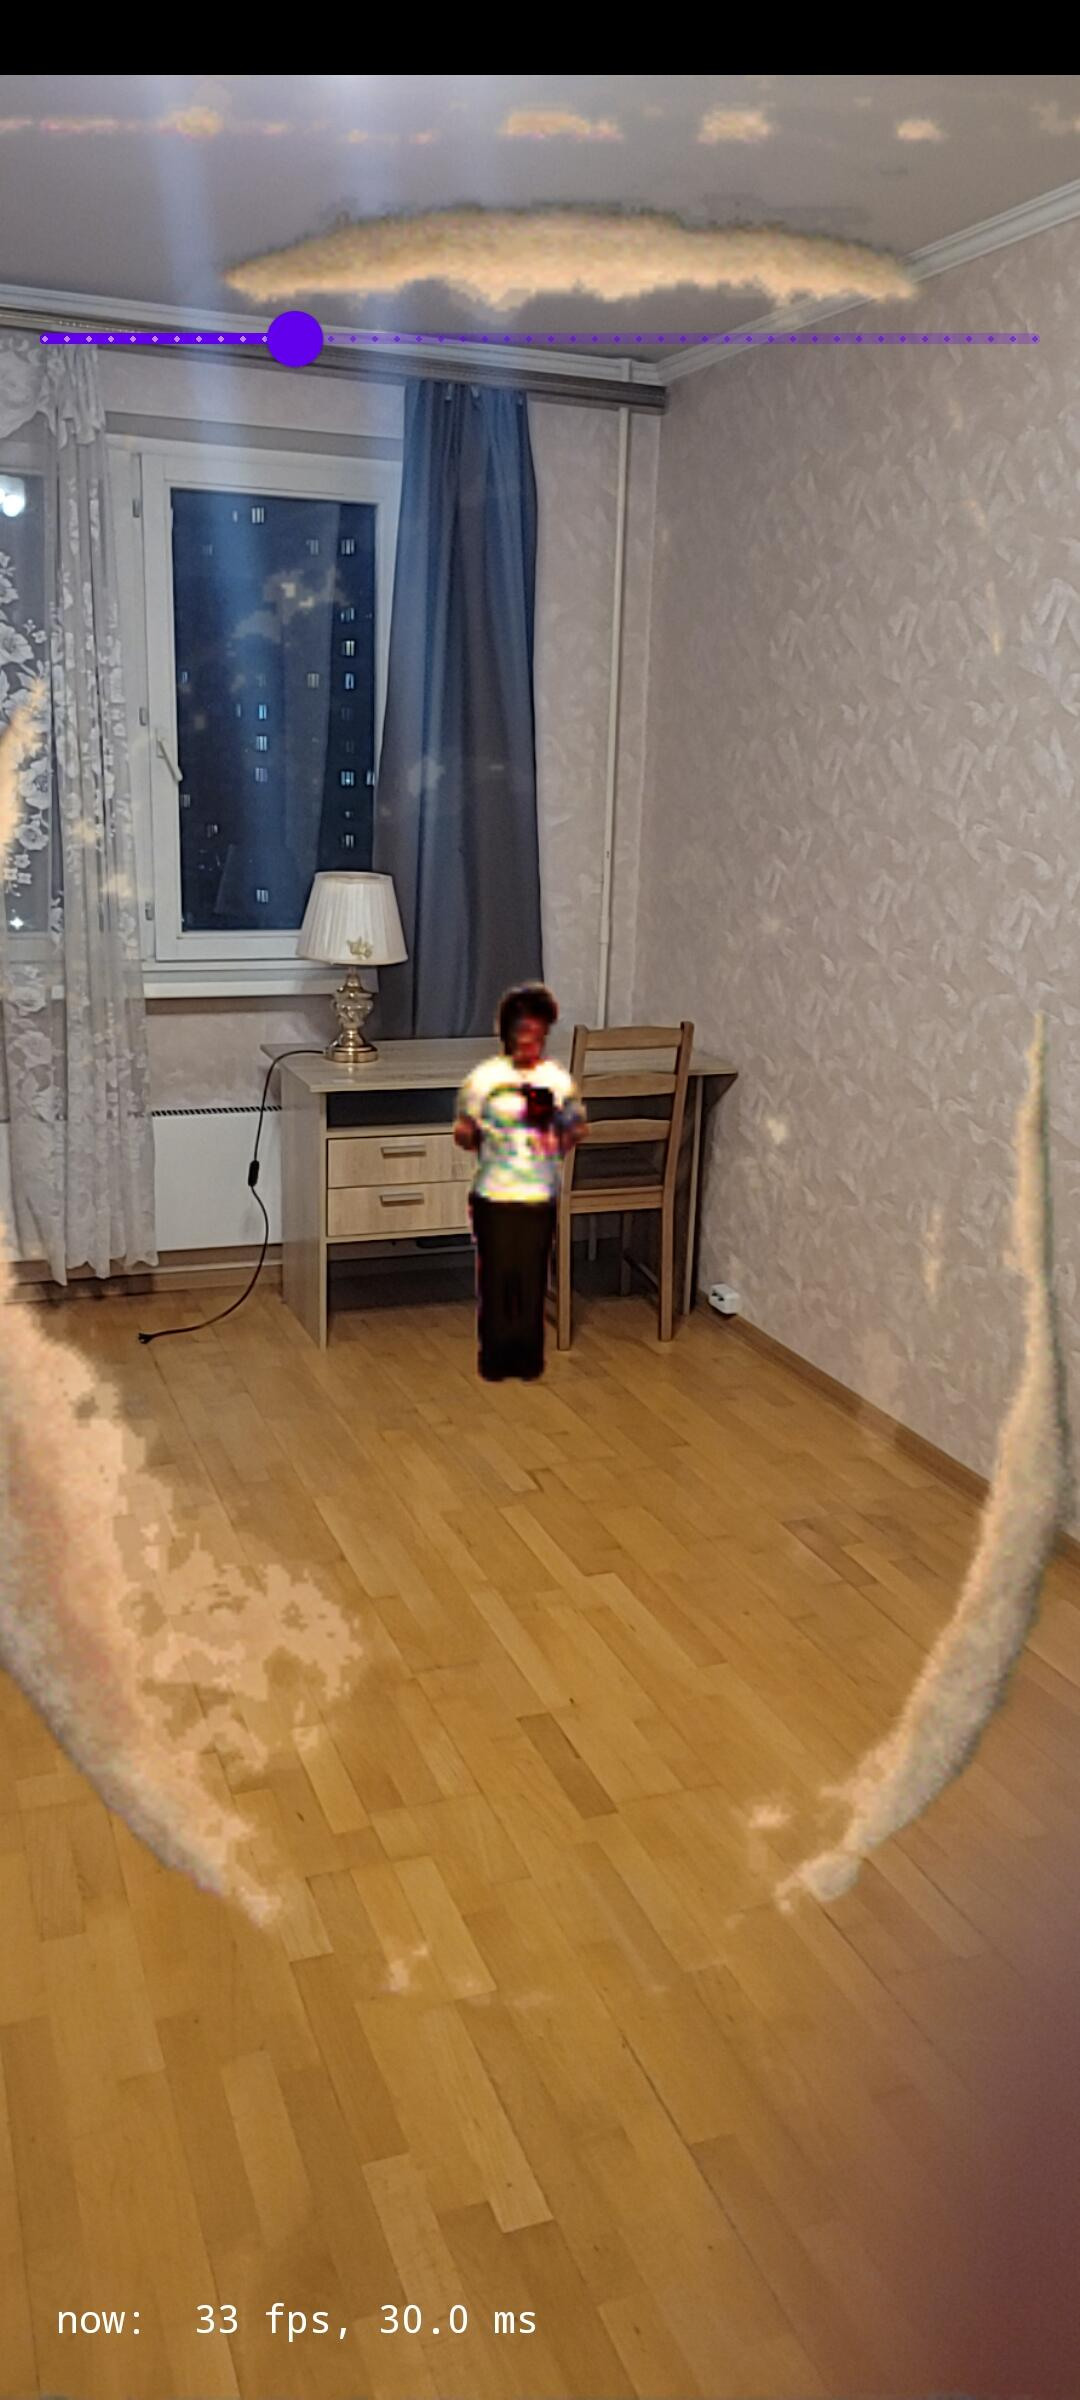
\includegraphics[width=\linewidth]{\imgfp/mobile_screenshots/far-away-screen-crop}%
		\caption{}
		\label{fig:far_screen_crop}
	\end{subfigure}
	\hfill
	\begin{subfigure}[b]{0.32\textwidth}
		\centering
		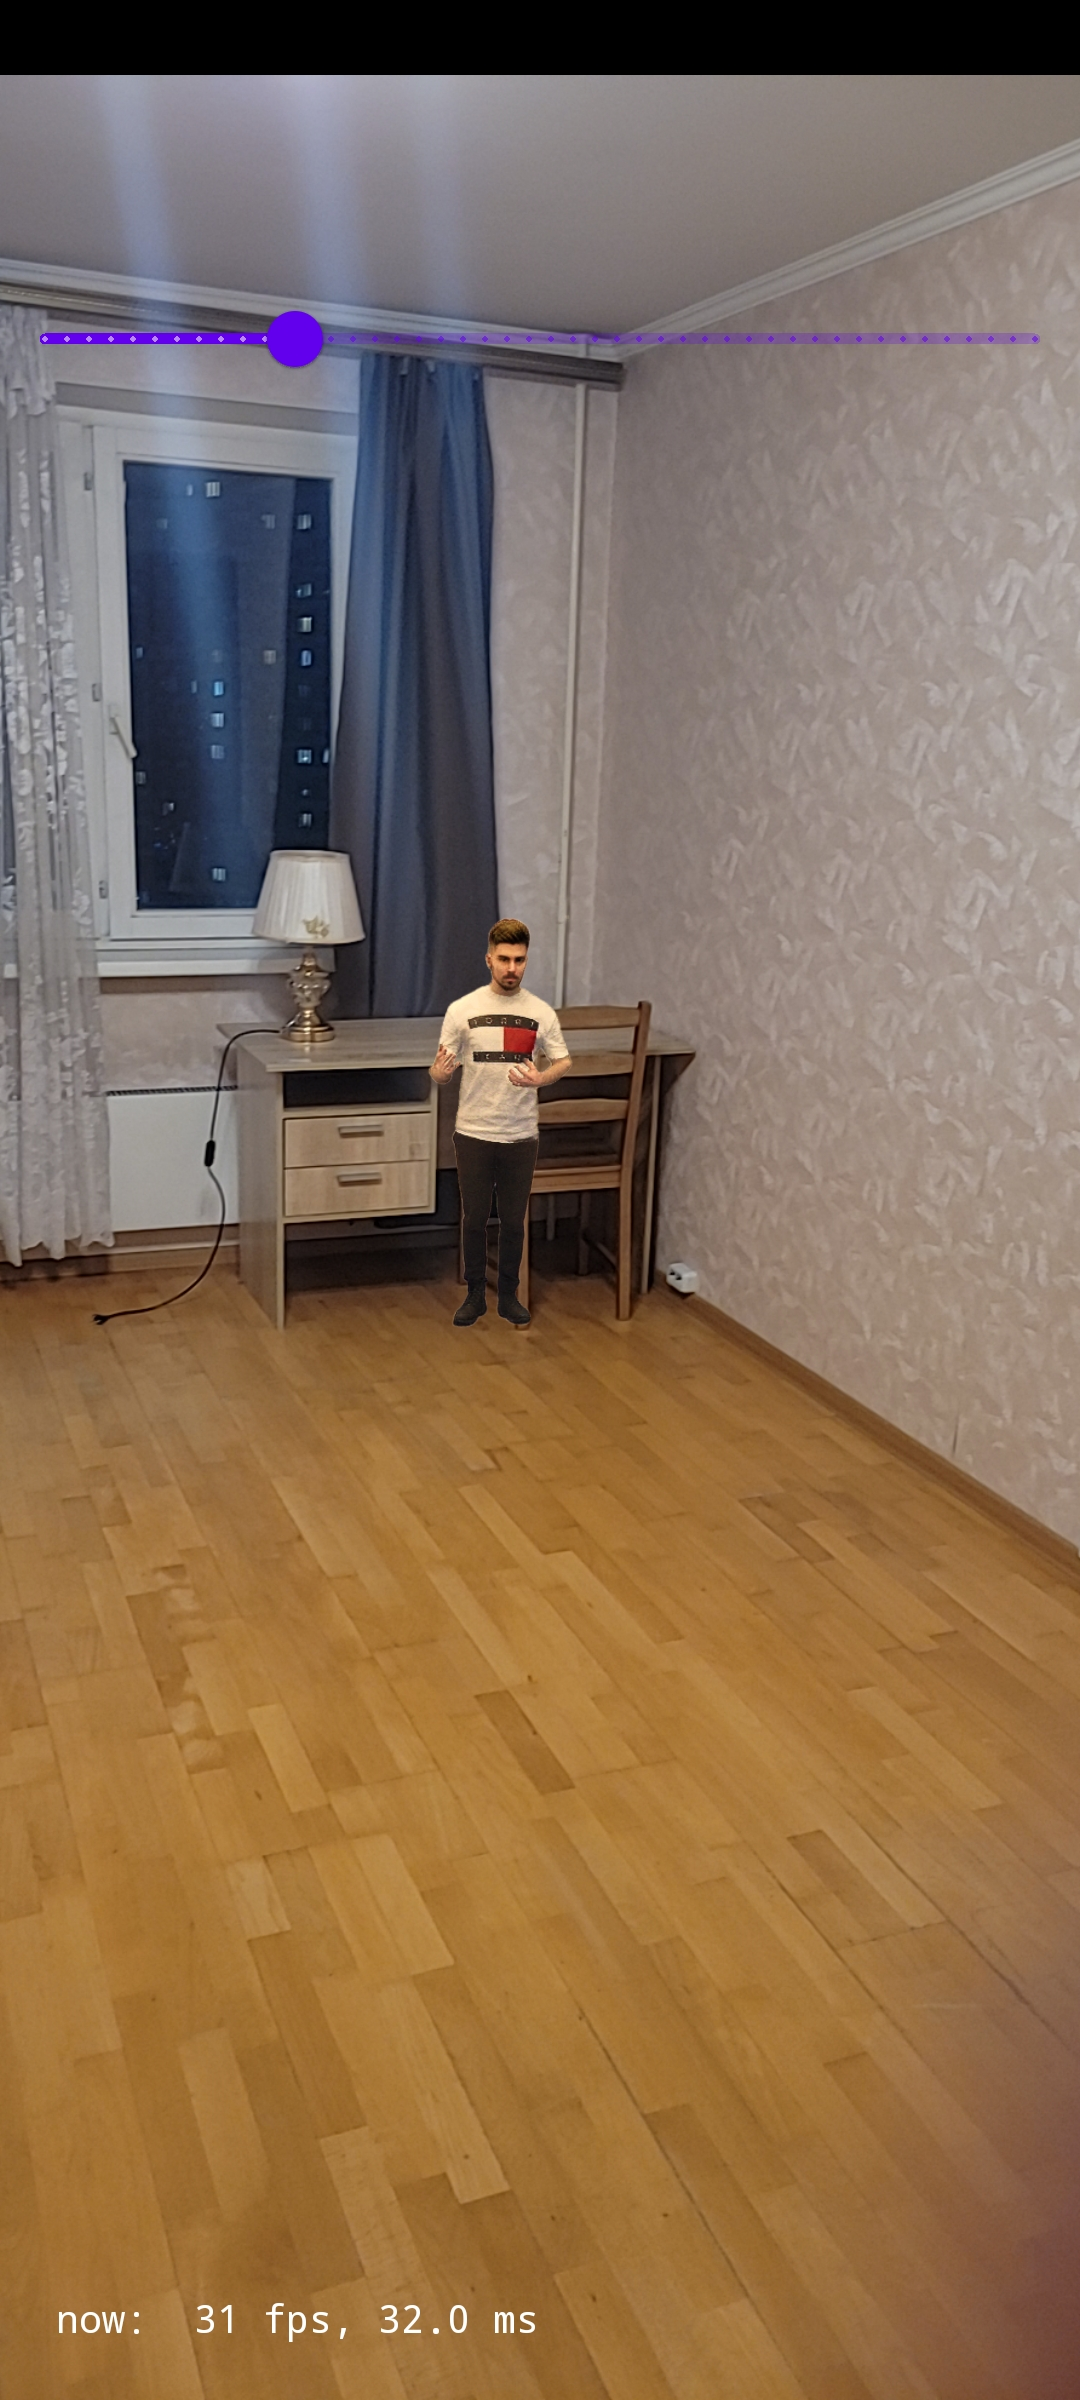
\includegraphics[width=\linewidth]{\imgfp/mobile_screenshots/far-away-crop}
		\caption{}
		\label{fig:far_dynamic_crop}
	\end{subfigure}
	\hfill
	\begin{subfigure}[b]{0.32\textwidth}
		\centering
		\includegraphics[width=\linewidth]{\imgfp/mobile_screenshots/far-away-crop-debug}
		\caption{}
		\label{fig:far_dynamic_crop_debug}
	\end{subfigure}
	\caption{Comparison of projection modes. (\protect\subref{fig:far_screen_crop}) A projection matrix that spans the whole screen (default mode). Since the input image is square in our pipeline, the input image is effectively much wider than the screen, and most of the generated image is wasted. Moreover, the input contains a tiny rasterization of the mesh, and unless the neural network was trained to see such small inputs, it may produce visual artifacts, as shown. (\protect\subref{fig:far_dynamic_crop}) A dynamic crop approach used in this work maximizes the avatar in the input rasterization, thus the network produces an image of sufficient quality. (\protect\subref{fig:far_dynamic_crop_debug}) Shows the output image without a segmentation mask applied, allowing us to see the borders of the dynamic crop. It covers all the joints and expands or shrinks on every frame.}
	\label{fig:far_examples}
\end{figure}
\begin{figure}
	%\fboxrule=2pt
	\centering
	\begin{subfigure}[b]{0.32\textwidth}
		\centering
		\includegraphics[width=\linewidth]{\imgfp/mobile_screenshots/crop-joints}%
		\caption{}
		\label{fig:zoom_inefficient_crop}
	\end{subfigure}
	\hfill
	\begin{subfigure}[b]{0.32\textwidth}
		\centering
		\includegraphics[width=\linewidth]{\imgfp/mobile_screenshots/screen-proj}
		\caption{}
		\label{fig:zoom_screen_crop}
	\end{subfigure}
	\hfill
	\begin{subfigure}[b]{0.32\textwidth}
		\centering
		\includegraphics[width=\linewidth]{\imgfp/mobile_screenshots/crop-custom}
		\caption{}
		\label{fig:zoom_smallest_crop}
	\end{subfigure}
	\caption{Comparison of projection modes in close view. (\protect\subref{fig:zoom_inefficient_crop}) A projection matrix that spans the whole screen (default mode). Even if the avatar spans almost the whole screen, parts of the frame are still being wasted, decreasing the possible resolution of the avatar. (\protect\subref{fig:zoom_screen_crop}) A dynamic crop around all the joints. A bit higher quality in this scenario, but the crop is similar to full-screen projection. (\protect\subref{fig:zoom_smallest_crop}) A dynamic crop around only seen body parts. Yields the highest quality, since it minimizes the area of wasted space.}
	\label{fig:zoom_examples}
\end{figure}

%\setkeys{Gin}{draft=false}

\begin{figure}
	\centering
	\includegraphics[width=\textwidth]{\imgfp/profiler/512_4x4_bn_res_print}
	\caption{Qualcomm Snapdragon Profiler output of hardware metrics, for 9 frames of a neural renderer inference on mobile. Configuration: $512\times512$ resolution, ResNet18 encoder, Batch Normalization layers, 16 input channels are generated as 4 OpenGL textures (thus rearranged in memory on each frame). Look at the first orange row "CDSP Utilization" indicating moments when DSP was either inferring or idle. Most of the time, the GPU work (of generating the input frame) takes place at the same time as the inference of the previous frame. This implicit parallelization by the device reduces overall idleness. However, out of 9 frames, 2 have twice as higher idleness on the DSP. These moments might correlate with row "L2 DU Read miss" (3rd from the end), indicating that due to inefficient memory layout, it may fit memory caches worse and "choke" on waiting for the arrival of the data.}
	\label{fig:profiler_4x4_bn_res}
\end{figure}

\begin{figure}
	\centering
	\includegraphics[width=\textwidth]{\imgfp/profiler/512_16_bn_res_print}
	\caption{Qualcomm Snapdragon Profiler output of hardware metrics, for 9 frames of a neural renderer inference on mobile. Configuration: $512\times512$ resolution, ResNet18 encoder, Batch Normalization layers, 16 input channels are generated as 1 OpenGL texture packed with quantized values. It is an efficient memory layout for generating the input frame of the DNN, that doesn't require additional rearrangement in memory. Unlike the previous figure, now the row "L2 DU Read miss" (3rd from the end) shows a lot fewer misses of memory caches, when inferring the DNN on DSP. This decreases the inference time, as reported in Table \ref{tab:mobile-performance}.}
	\label{fig:profiler_16_bn_res}
\end{figure}

\begin{figure}
	\centering
	\includegraphics[width=\textwidth]{\imgfp/profiler/512_16_bn_mv2_print}
	\caption{Qualcomm Snapdragon Profiler output of hardware metrics, for 9 frames of a neural renderer inference on mobile. Configuration: $512\times512$ resolution, MobileNetV2 encoder, Batch Normalization layers, 16 input channels are generated as 1 OpenGL texture packed with quantized values. The MobileNetV2 in theory should drastically outperform ResNet18 (which we use in this work by default). However, as we observe, the performance is roughly similar (See Table \ref{tab:mobile-performance}). In terms of DSP hardware utilization seen on this figure (orange rows), no apparent difference with ResNet is seen, except for smaller values in the "DCache Store miss" row, indicating that intermediate data is written into memory in such a way to use adjacent memory addresses as long as possible, which improves utilization of memory caches and should improve performance. We speculate, that it's just that depth-wise convolution operations used in MobileNetV2 have a fairly inefficient implementation on the target DSP hardware.}
	\label{fig:profiler_16_bn_mv2}
\end{figure}

\begin{figure}
	\centering
	\includegraphics[width=\textwidth]{\imgfp/profiler/512_16_in_res_print}
	\caption{Qualcomm Snapdragon Profiler output of hardware metrics, for 9 frames of a neural renderer inference on mobile. Configuration: $512\times512$ resolution, ResNet18 encoder, Instance Normalization layers, 16 input channels are generated as 1 OpenGL texture packed with quantized values. The only notable difference in DSP utilization (orange rows), compared to the above figures, is in the "Packets executed" row (fifth from the end). It shows much higher values than in figure \ref{fig:profiler_16_bn_res} with Batch Normalization layers. This correlates with the fact, that Instance Normalization layers simply require more computations than Batch Normalizations (where tensor statistics are pre-computed), leading to worse performance, as reported in Table \ref{tab:mobile-performance}.}
	\label{fig:profiler_16_in_res}
\end{figure}

\clearpage
\newpage

%\setkeys{Gin}{draft=false}
\section{Experiments on DNN training}
\label{appb:exps}

Firstly, we present a table of training losses and validation metrics for the experiments. The experiments are sorted by validation metrics from best to worst. The Top-5 metric values are emphasized with a bold underlined font, and the best value of all is additionally colored in blue. We notate the table columns: the "GAN G" is Adversarial loss of the Generator, the "GAN D-R" is Adversarial loss of the Discriminator on real images, and the "GAN D-F" is Adversarial loss of the Discriminator on synthesized (fake) images. We shorten the description of experiments, where Batch normalization layers do not collect running batch statistics on zoomed frames, as "no zoom stats BN". Next, we demonstrate most of the experiments as collations of training and test images, as well as plots of training losses and plots of validation metrics. We show images synthesized on training epochs with the best visual quality (visually assessed). Images encased with a gray border are \textit{synthesized}, the border-less images are ground truth. Each column of the images has a colored mark at the bottom. It represents a corresponding line color on the plots for the given experiment. Each page includes a legend with a short description of the experimental setup and adjustments. To shorten the descriptions, we use a notation like $\Omega=$ to show that any other usage of $\Omega$ on the same plot uses or extends from this experiment. We use notation $\nabla=0$ a few times, which means only those values in analytic gradient tensors that are very close to 0.

The images were compressed to reduce the file size of this manuscript (from almost a gigabyte, to a few megabytes). This may affect the quality of the images. The originally synthesized images are sharper and less noisy. On the other hand, the general visual artifacts are mostly preserved. As a minimal subset of training images, we show full-body and upper body frames with the most difficult poses available, frames from front and back, as well as a close-up shot of a face. The selected test frames consist of views: of the bottom of the shoes -- showing artifacts for the body parts that were unseen during training; of a face close-up -- may lose similarity with the person's face due to overfitting; of top-down, which may show overfitting to the frames in the training set, where the person bends forward, and a shadow is cast upon their upper body (see training images, first row); of the upper-body, to compare the clarity of T-shirt ornaments, which may be lost due to possible misalignment of the ground truth images and the body model \cite{dnn:smplx19}, because of which neural texture pixels may fit different locations on the body.

To keep this section compact, we omit from the table experiments, that were trained on non-default train sequences or resulted in a severe visual quality downgrade (although the images will be presented). We demonstrate only a subset of loss and metric curves, namely LPIPS, L1, MS-SSIM, and adversarial losses. A single plot of the adversarial loss will combine two lines: the generator's loss (solid line) is the accuracy of the discriminator on the synthesized images, and the discriminator's loss (translucent line with colored dots) is the accuracy of the discriminator on the real images. The former should decrease, indicating that the generator produces plausible images, and the latter should increase, indicating that the discriminator learns the realism of ground truth images.

%\clearpage
%\newpage
\begin{table}[!h]
	\renewcommand{\arraystretch}{0.25}
	\linespread{0.25}\selectfont\centering\small
	\setlength\tabcolsep{1.5pt}
	\rowcolors{2}{gray!15}{white}
	\caption{Training losses for the performed experiments}
	\label{tab:training-losses}
	\begin{tabularx}{\textwidth}{>{\centering\arraybackslash}X|c|c|c|c|c|c|c}\hline
		\rowcolor{white}
		\textbf{Experiment} & {\footnotesize\textbf{\thead{GAN\\G↓}}} & {\footnotesize\textbf{\thead{GAN\\D-R↑}}} & {\footnotesize\textbf{\thead{GAN\\D-F↑}}} & {\footnotesize\textbf{\thead{FM↓\\$\cdot10^2$}}} & {\footnotesize\textbf{\thead{L1↓\\$\cdot10^3$}}} & {\footnotesize\textbf{\thead{Dice↓\\$\cdot10^3$}}} & {\footnotesize\textbf{\thead{LPIPS↓\\$\cdot10^2$}}}\\\hline
		\thead[l]{1. Baseline, add camera-space augmentations \textsuperscript{Fig.\ref{fig:exp:baselines}}}
		& 0.58 & 0.88 & 0.94 & 37.77 & \textbf{\underline{9.93}} & \textbf{\underline{1.91}} & \textbf{\underline{11.19}} \\ % vA01_e05_50
		\thead[l]{2. Baseline, add camera-space,\\\-\quad\quad horizontal flip augment \textsuperscript{Fig.\ref{fig:exp:baselines}}}
		& 0.56 & 0.88 & 1.32 & 37.84 & \textbf{\underline{10.43}} & 2.32 & \textbf{\underline{10.60}} \\ % vA01_e05_50_flips
		\thead[l]{3. No GAN losses on zooms \textsuperscript{Fig.\ref{fig:exp:scale-distr-enable-disable-stat-or-gan}}}
		& 0.56 & 0.91 & 0.95 & 29.16 & 13.19 & 3.20 & 12.95 \\ % vA03_03_znod
		\thead[l]{4. Baseline, resolution $512\times512$ \textsuperscript{Fig.\ref{fig:exp:baselines}}}
		& 0.56 & 0.85 & 1.64 & 33.94 & \textbf{\underline{8.05}} & \textbf{\underline{1.58}} & \textbf{\underline{8.94}} \\ % v05_50
		\thead[l]{5. Instance normalizations instead of BN \textsuperscript{Fig.\ref{fig:exp:different-norms}}}
		& 0.45 & 1.23 & 1.03 & 36.89 & 13.48 & 4.41 & 14.25 \\ % A01_07_ai
		\thead[l]{6. No GAN losses on FB images \textsuperscript{Fig.\ref{fig:exp:scale-distr-enable-disable-stat-or-gan}}}
		& \textbf{\underline{0.30}} & 1.07 & 1.08 & 42.37 & 12.76 & 3.42 & 12.57 \\ % vA03_03_fbnod
		\thead[l]{7. Zoom on joints up to x12,\\\-\quad\quad full-body is more probable \textsuperscript{Fig.\ref{fig:exp:a03-bl}}}
		& 0.48 & 1.05 & 1.04 & 45.70 & 17.20 & 3.70 & 14.16 \\ % vA03_01_nobnf
		\thead[l]{8. Noise augmentation $\sigma=0.02$ on neural texture \textsuperscript{Fig.\ref{fig:exp:add-noise-ntex}}}
		& 0.46 & 1.07 & 1.12 & 47.55 & 19.70 & 3.71 & 14.73 \\ % A03_06_ntex002
		\thead[l]{9. All losses with equal weights \textsuperscript{Fig.\ref{fig:exp:loss-weights}}}
		& 0.52 & 0.81 & 0.85 & 36.30 & 22.89 & 5.01 & 22.30 \\ % A01_53_1
		\thead[l]{10. Noise augmentation $\sigma=0.1$ on input tensor \textsuperscript{Fig.\ref{fig:exp:add-noise-input}}}
		& 0.46 & 1.19 & 1.09 & 49.95 & 20.14 & 4.05 & 14.32 \\ % A03_06_inp01
		\thead[l]{11. Noise augmentation $\sigma=0.01$ on input tensor \textsuperscript{Fig.\ref{fig:exp:add-noise-input}}}
		& 0.45 & 1.09 & 1.03 & 47.64 & 19.04 & 3.64 & 13.42 \\ % A03_06_inp001
		\thead[l]{12. Noise augmentation $\sigma=0.02$ on input tensor \textsuperscript{Fig.\ref{fig:exp:add-noise-input}}}
		& 0.44 & 1.08 & 1.00 & 49.54 & 18.92 & 3.69 & 14.54 \\ % A03_06_inp002
		\thead[l]{13. Discriminator w/o normalization layers \textsuperscript{Fig.\ref{fig:exp:nonorm:d:rd:rhead}}}
		& 0.53 & 0.80 & 1.00 & \textcolor{blue}{\textbf{\underline{1.46}}} & 25.86 & 3.67 & 20.11 \\ % A01_37_nodisnorm
		\thead[l]{14. Dropout $p=0.1$ in encoder layers \textsuperscript{Fig.\ref{fig:exp:dropout-e-d}}}
		& 0.46 & 1.18 & 1.03 & 51.76 & 22.12 & 5.25 & 17.11 \\ % A03_04_01e
		\thead[l]{15. Zoom on vertices, selected with equal probability \textsuperscript{Fig.\ref{fig:exp:zoom-vertices}}}
		& 0.46 & 1.16 & 1.24 & 42.64 & 25.16 & 3.52 & 19.05 \\ % A01_30_ai
		\thead[l]{16. Noise augmentation $\sigma=0.01$ on neural texture \textsuperscript{Fig.\ref{fig:exp:add-noise-input}}}
		& 0.44 & 1.09 & 1.11 & 44.68 & 19.49 & 3.96 & 15.50 \\ % A03_06_ntex001
		\thead[l]{17. Gradient clip discriminator to mean norm \textsuperscript{Fig.\ref{fig:exp:gradclip-constant-or-mean}}}
		& 0.45 & 1.07 & 1.08 & 44.48 & 25.62 & 4.01 & 19.88 \\ % A01_35_dis_d1_01
		\thead[l]{18. Encoder 25\% fewer parameters \textsuperscript{Fig.\ref{fig:exp:neural-renderer-capacity}}}
		& 0.43 & 0.97 & 1.09 & 38.94 & 26.47 & \textbf{\underline{1.98}} & 21.19 \\ % A01_27_enc2221
		\thead[l]{19. Gradient clip renderer to 5 norm \textsuperscript{Fig.\ref{fig:exp:gradclip-constant-or-mean}}}
		& 0.43 & 1.16 & 1.27 & 41.06 & 23.31 & 4.34 & 18.50 \\ % A01_35_5_01
		\thead[l]{20. Gradient clip renderer to mean$\times0.5$ norm \textsuperscript{Fig.\ref{fig:exp:gradclip-mean-fraction}}}
		& 0.43 & 1.27 & 1.09 & 45.93 & 21.33 & 4.29 & 18.85 \\ % A01_35_d2_01
		\thead[l]{21. Weight decay $10^{-3}$ renderer/discriminator \textsuperscript{Fig.\ref{fig:exp:wdecay-nr3:ntex+disc}}}
		& 0.48 & 1.18 & 1.15 & 45.38 & 17.69 & 3.52 & 17.61 \\ % A03_07_nr3_d3
		\thead[l]{22. Noise augmentation $\sigma=0.01$ on neural texture \textsuperscript{Fig.\ref{fig:exp:add-noise-ntex}}}
		& 0.47 & 1.19 & 1.09 & 53.14 & 19.50 & 4.60 & 17.24 \\ % A03_06_ntex01
		\thead[l]{23. Weight decay $10^{-2}$ renderer/discriminator/texture \textsuperscript{Fig.\ref{fig:exp:wdecay-nr2:ntex2+disc}}}
		& 0.46 & 1.21 & 1.15 & 42.81 & 22.16 & 2.97 & 16.65 \\ % A03_07_nr2_d2_ntex2
		\thead[l]{24. Neural texture's learning rate $\times5$ \textsuperscript{Fig.\ref{fig:exp:ntex-lr-higher}}}
		& 0.40 & 1.10 & 1.06 & 48.54 & 24.38 & 3.42 & 19.67 \\ % A01_39_ntex5
		\thead[l]{25. Pass input tensor to inner layers of encoder \textsuperscript{Fig.\ref{fig:exp:pass-input-in-encoder}}}
		& 0.45 & 1.15 & 1.09 & 44.48 & 22.04 & 3.40 & 17.88 \\ % A01_38_cat
		\thead[l]{26. Weight decay $10^{-3}$ renderer \textsuperscript{Fig.\ref{fig:exp:wdecay-nr3:ntex+disc}}}
		& 0.48 & 1.19 & 1.31 & 43.32 & 18.98 & 3.20 & 16.86 \\ % A03_07_nr3
		\thead[l]{27. Decoder 50\% fewer parameters \textsuperscript{Fig.\ref{fig:exp:neural-renderer-capacity}}}
		& 0.41 & 1.13 & 1.03 & 42.69 & 21.49 & 3.00 & 19.75 \\ % A01_27_dec50pct
		\thead[l]{28. Zoom on vertices, prioritize person's head \textsuperscript{Fig.\ref{fig:exp:zoom-vertices}}}
		& 0.45 & 1.16 & 1.06 & 45.07 & 24.04 & 3.66 & 21.23 \\ % A01_29_ai
		\thead[l]{29. Gradient clip renderer to mean$\times0.2$ norm \textsuperscript{Fig.\ref{fig:exp:gradclip-mean-fraction}}}
		& 0.46 & 1.20 & 1.45 & 43.52 & 24.49 & 3.86 & 18.74 \\ % A01_35_d5_01
		\thead[l]{30. Gradient clip renderer to mean norm \textsuperscript{Fig.\ref{fig:exp:gradclip-mean-fraction}}}
		& 0.51 & 1.07 & 1.14 & 48.25 & 21.74 & 4.12 & 19.09 \\ % A01_35_d1_01
	\end{tabularx}
\end{table}\clearpage\newpage
\begin{table}
	\renewcommand{\arraystretch}{0.25}
	\linespread{0.25}\selectfont\centering\small
	\setlength\tabcolsep{1.5pt}
	\rowcolors{2}{gray!15}{white}
	\caption*{\textit{(continuation of Table \ref{tab:training-losses})}}
	\begin{tabularx}{\textwidth}{>{\centering\arraybackslash}X|c|c|c|c|c|c|c}\hline
		\rowcolor{white}
		\textbf{Experiment} & {\footnotesize\textbf{\thead{GAN\\G↓}}} & {\footnotesize\textbf{\thead{GAN\\D-R↑}}} & {\footnotesize\textbf{\thead{GAN\\D-F↑}}} & {\footnotesize\textbf{\thead{FM↓\\$\cdot10^2$}}} & {\footnotesize\textbf{\thead{L1↓\\$\cdot10^3$}}} & {\footnotesize\textbf{\thead{Dice↓\\$\cdot10^3$}}} & {\footnotesize\textbf{\thead{LPIPS↓\\$\cdot10^2$}}}\\\hline
		\thead[l]{31. Weight decay $10^{-5}$ renderer \textsuperscript{Fig.\ref{fig:exp:wdecay-nr654}}}
		& 0.43 & 1.20 & 1.14 & 46.83 & 19.53 & 4.03 & 15.83 \\ % A03_07_nr5
		\thead[l]{32. Weight decay $10^{-2}$ renderer/discriminator,\\\-\quad\quad $10^{-1}$ for texture \textsuperscript{Fig.\ref{fig:exp:wdecay-nr2:ntex1+disc}}}
		& 0.41 & 1.11 & 1.35 & 42.14 & 20.21 & 3.83 & 17.92 \\ % A03_07_nr2_d2_ntex1
		\thead[l]{33. Replace a few channels of encoder's inner layers\\\-\quad\quad with an input tensor \textsuperscript{Fig.\ref{fig:exp:pass-input-in-encoder}}}
		& 0.43 & 1.07 & 1.13 & 49.04 & 19.83 & 3.85 & 18.28 \\ % A01_38_ai
		\thead[l]{34. Neural texture's learning rate $\times10$ \textsuperscript{Fig.\ref{fig:exp:ntex-lr-higher}}}
		& 0.44 & 1.08 & 1.09 & 48.74 & 18.06 & 3.90 & 13.50 \\ % A01_39_ntex10
		\thead[l]{35. Weight decay $10^{-2}$ renderer \textsuperscript{Fig.\ref{fig:exp:wdecay-nr432}}}
		& 0.38 & 1.18 & 1.08 & 41.50 & 20.94 & 3.61 & 16.68 \\ % A03_07_nr2
		\thead[l]{36. Equal loss weights + higher texture learning rate \textsuperscript{Fig.\ref{fig:exp:loss-weights}}}
		& 0.59 & 0.81 & 0.90 & 33.03 & 22.19 & 3.78 & 20.14 \\ % A01_53_ntexlr
		\thead[l]{37. Zoom on vertices with equal probability,\\\-\quad\quad zoom scale is mostly full-body \textsuperscript{Fig.\ref{fig:exp:a03-bl}}}
		& 0.40 & 1.07 & 1.22 & 46.77 & 18.99 & 4.50 & 14.83 \\ % vA03_01_nobnf_ut
		\thead[l]{38. Strong affine translation \textsuperscript{Fig.\ref{fig:exp:strong-affine-aug}}}
		& 0.46 & 1.18 & 1.07 & 49.83 & 22.89 & 4.32 & 17.15 \\ % vA01_03_vt
		\thead[l]{39. Gradient clip renderer to 2 norm \textsuperscript{Fig.\ref{fig:exp:gradclip-constant-or-mean}}}
		& 0.39 & 1.18 & 1.18 & 42.27 & 22.66 & 4.19 & 19.53 \\ % A01_35_2_01
		\thead[l]{40. Weight decay $10^{-2}$ renderer,\\\-\quad\quad $10^{-1}$ for texture/discriminator \textsuperscript{Fig.\ref{fig:exp:wdecay-nr2:ntex1+disc}}}
		& 0.39 & 1.16 & 1.03 & 48.79 & 15.23 & 3.97 & 15.79 \\ % A03_07_nr2_d1_ntex1
		\thead[l]{41. Texture optimizer's state does not update if $\nabla=0$ \textsuperscript{Fig.\ref{fig:exp:nza-or-bnfix}}}
		& 0.44 & 1.02 & 1.16 & 48.58 & 17.18 & 4.30 & 18.70 \\ % A01_31_ai
		\thead[l]{42. LR scheduler with warmup,\\\-\quad\quad gradient clip renderer to 10 norm \textsuperscript{Fig.\ref{fig:exp:gradclip-scheduler}}}
		& 0.47 & 1.03 & 1.16 & 46.70 & 19.77 & 4.16 & 19.49 \\ % A01_42_lr2m6_gc10
		\thead[l]{43. Weight decay $10^{-4}$ renderer \textsuperscript{Fig.\ref{fig:exp:wdecay-nr654}}}
		& 0.37 & 1.08 & 1.17 & 45.94 & 20.77 & 3.34 & 16.26 \\ % A03_07_nr4
		\thead[l]{44. Weight decay $10^{-6}$ renderer \textsuperscript{Fig.\ref{fig:exp:wdecay-nr654}}}
		& 0.45 & 1.14 & 1.18 & 45.95 & 19.66 & 3.87 & 14.58 \\ % A03_07_nr6
		\thead[l]{45. Renderer's last layers w/o normalization layers \textsuperscript{Fig.\ref{fig:exp:nonorm:d:rd:rhead}}}
		& 0.50 & 1.15 & 1.21 & 43.62 & 21.65 & 3.81 & 19.93 \\ % A01_37_noheadnorm
		\thead[l]{46. Renderer and discriminator's BN layers\\\-\quad\quad w/o learned affine parameters \textsuperscript{Fig.\ref{fig:exp:norm-noaffine}}}
		& 0.48 & 1.11 & 1.16 & 48.05 & 25.22 & 3.95 & 17.84 \\ % A01_43_03v_rd
		\thead[l]{47. Dropout $p=0.1$ in encoder after convolutions \textsuperscript{Fig.\ref{fig:exp:dropout-all-conv-ed-ed}}}
		& 0.41 & 1.12 & 1.02 & 50.83 & 19.58 & 5.19 & 17.27 \\ % A03_04_c01e
		\thead[l]{48. LR scheduler with warmup \textsuperscript{Fig.\ref{fig:exp:gradclip-scheduler}}}
		& 0.44 & 1.15 & 1.09 & 46.67 & 20.97 & 4.07 & 19.21 \\ % A01_42_lr2m6
		\thead[l]{49. Renderer's BN layers w/o learned affine parameters \textsuperscript{Fig.\ref{fig:exp:norm-noaffine}}}
		& 0.47 & 1.06 & 1.27 & 50.03 & 20.41 & 3.34 & 20.62 \\ % A01_43_03v_r
		\thead[l]{50. Zoom on vertices with equal probability,\\\-\quad\quad no zoom stats BN \textsuperscript{Fig.\ref{fig:exp:nza-bnfix-zoomvertices}}}
		& 0.36 & 1.25 & 1.59 & 44.42 & 15.87 & 4.50 & 14.03 \\ % vA01_24
		\thead[l]{51. Zoom on vertices with equal probability,\\\-\quad\quad mostly full-body input, no zoom stats BN \textsuperscript{Fig.\ref{fig:exp:a03-uniform}}}
		& \textbf{\underline{0.28}} & \textbf{\underline{1.51}} & \textbf{\underline{1.78}} & 45.22 & 15.31 & 5.10 & 14.35 \\ % vA03_01_uniform
		\thead[l]{52. Weight decay $10^{-3}$ renderer/discriminator/texture \textsuperscript{Fig.\ref{fig:exp:wdecay-nr3:ntex+disc}}}
		& 0.42 & 1.26 & 1.19 & 48.55 & 21.09 & 3.06 & 14.78 \\ % A03_07_nr3_d3_ntex3
		\thead[l]{53. Neural texture 8 channels, not 16 \textsuperscript{Fig.\ref{fig:exp:nza-or-ntex8}}}
		& 0.49 & 1.10 & 1.04 & 47.85 & 25.88 & 3.84 & 18.18 \\ % A01_33_ai
		\thead[l]{54. LR scheduler with warmup,\\\-\quad\quad gradient clip renderer to 20 norm \textsuperscript{Fig.\ref{fig:exp:gradclip-scheduler}}}
		& 0.44 & 1.10 & 1.00 & 48.72 & 25.09 & 4.02 & 19.47 \\ % A01_42_lr2m6_gc20
		\thead[l]{55. Zooms on joints x4.5 \textsuperscript{Fig.\ref{fig:exp:basic-zooms}}}
		& 0.41 & 1.03 & 1.15 & 48.69 & 24.51 & 4.21 & 20.20 \\ % A01_03_ai_retrain_val
		\thead[l]{56. Dropout $p=0.05$ in renderer layers \textsuperscript{Fig.\ref{fig:exp:dropout-ed-ed}}}
		& 0.42 & 1.07 & 1.41 & 56.26 & 21.35 & 6.00 & 17.40 \\ % A03_04_005ed
		\thead[l]{57. Zoom to vertices with equal probability,\\\-\quad\quad mostly full-body input \textsuperscript{Fig.\ref{fig:exp:a03-bl}}}
		& 0.46 & 1.40 & 1.17 & 48.61 & 23.19 & 3.80 & 17.70 \\ % A03_01_bl
		\thead[l]{58. Weight decay $10^{-2}$ renderer/texture,\\\-\quad\quad $10^{-1}$ for discriminator \textsuperscript{Fig.\ref{fig:exp:wdecay-nr2:ntex2+disc}}}
		& 0.40 & 1.11 & 1.16 & 42.80 & 20.00 & 3.38 & 17.32 \\ % A03_07_nr2_d1_ntex2
		\thead[l]{59. Weight decay $10^{-1}$ renderer \textsuperscript{Fig.\ref{fig:exp:wdecay-nr2:nronly}}}
		& 0.45 & 1.25 & 1.12 & 46.20 & 23.79 & 3.12 & 18.10 \\ % A03_07_nr1
		\thead[l]{60. Neural texture 8 channels, no zoom stats BN,\\\-\quad\quad texture optimizer's state does not update if $\nabla=0$ \textsuperscript{Fig.\ref{fig:exp:nza-bnfix-ntex8}}}
		& 0.37 & 1.04 & \textcolor{blue}{\textbf{\underline{1.91}}} & 43.76 & 15.49 & 5.13 & 14.74 \\ % vA01_28
	\end{tabularx}
\end{table}\clearpage\newpage
\begin{table}
	\renewcommand{\arraystretch}{0.25}
	\linespread{0.25}\selectfont\centering\small
	\setlength\tabcolsep{1.5pt}
	\rowcolors{2}{gray!15}{white}
	\caption*{\textit{(continuation of Table \ref{tab:training-losses})}}
	\begin{tabularx}{\textwidth}{>{\centering\arraybackslash}X|c|c|c|c|c|c|c}\hline
		\rowcolor{white}
		\textbf{Experiment} & {\footnotesize\textbf{\thead{GAN\\G↓}}} & {\footnotesize\textbf{\thead{GAN\\D-R↑}}} & {\footnotesize\textbf{\thead{GAN\\D-F↑}}} & {\footnotesize\textbf{\thead{FM↓\\$\cdot10^2$}}} & {\footnotesize\textbf{\thead{L1↓\\$\cdot10^3$}}} & {\footnotesize\textbf{\thead{Dice↓\\$\cdot10^3$}}} & {\footnotesize\textbf{\thead{LPIPS↓\\$\cdot10^2$}}}\\\hline
		\thead[l]{61. Strong affine translation and rotation \textsuperscript{Fig.\ref{fig:exp:strong-affine-aug}}}
		& 0.49 & 1.12 & 1.34 & 54.53 & 17.92 & 5.09 & 17.49 \\ % vA01_03_vtr
		\thead[l]{62. Zooms on joints x2.0 \textsuperscript{Fig.\ref{fig:exp:basic-zooms-2}}}
		& 0.33 & 1.04 & 1.16 & 48.68 & 19.26 & 3.85 & 18.29 \\ % vA01_04
		\thead[l]{63. Texture optimizer's state does not update if $\nabla=0$,\\\-\quad\quad all normalization layers are removed \textsuperscript{Fig.\ref{fig:exp:nonorm:d:rd:rhead}}}
		& 0.58 & 0.83 & 0.93 & \textbf{\underline{1.63}} & 26.69 & 4.60 & 17.89 \\ % A01_37_ai
		\thead[l]{64. Texture optimizer's state does not update\\\-\quad\quad if $\nabla=0$, no zoom stats BN \textsuperscript{Fig.\ref{fig:exp:nza-bnfix-zoomvertices}}}
		& 0.44 & 1.11 & 1.30 & 15.78 & 16.79 & 5.39 & 15.88 \\ % vA01_23
		\thead[l]{65. All normalization layers are removed \textsuperscript{Fig.\ref{fig:exp:different-norms}}}
		& 0.48 & 1.31 & 1.19 & 21.57 & 16.43 & 6.05 & 15.38 \\ % vA01_08
		\thead[l]{66. Zooms on limbs x8.0 \textsuperscript{Fig.\ref{fig:exp:basic-zooms-2}}}
		& 0.38 & 1.12 & 1.06 & 54.46 & 22.75 & 5.18 & 18.37 \\ % vA01_01
		\thead[l]{67. Zooms on joints x3.5 \textsuperscript{Fig.\ref{fig:exp:basic-zooms-2}}}
		& 0.42 & 1.03 & 1.04 & 48.62 & 20.33 & 3.44 & 17.79 \\ % vA01_05
		\thead[l]{68. Dropout $p=0.01$ in decoder layers \textsuperscript{Fig.\ref{fig:exp:dropout-e-d}}}
		& 0.39 & 1.22 & 1.13 & 59.68 & 18.84 & 5.80 & 17.75 \\ % A03_04_01d
		\thead[l]{69. No zoom stats BN for 20\% of frames \textsuperscript{Fig.\ref{fig:exp:bnf-disable-track}}}
		& 0.42 & 1.15 & 1.56 & 54.05 & 15.95 & 4.93 & 14.75 \\ % vA01_06_notrack2
		\thead[l]{70. Renderer BN w/o learned affine parameters,\\\-\quad\quad discriminator with Instance norms \textsuperscript{Fig.\ref{fig:exp:renderer-noaffinenorm}}}
		& 0.40 & 1.06 & 1.42 & 9.38 & 14.79 & 4.74 & 13.62 \\ % vA01_43_rdin
		\thead[l]{71. Neural texture 8 channels, no zoom stats BN \textsuperscript{Fig.\ref{fig:exp:nza-bnfix-ntex8}}}
		& 0.38 & 1.06 & 1.17 & 50.84 & 16.89 & 6.05 & 15.78 \\ % vA01_25
		\thead[l]{72. Group Normalization layers instead of BN \textsuperscript{Fig.\ref{fig:exp:different-norms}}}
		& 0.44 & 1.09 & 1.26 & 25.29 & 15.05 & 4.57 & 15.45 \\ % vA01_09
		\thead[l]{73. Texture optimizer's state does not update\\\-\quad\quad if $\nabla=0$, no normalizations in renderer \textsuperscript{Fig.\ref{fig:exp:nonorm:r:rd:r+dinstancenorm}}}
		& \textcolor{blue}{\textbf{\underline{0.25}}} & 1.36 & 1.65 & 58.29 & 26.52 & 4.94 & 21.41 \\ % A01_37_dis_bn
		\thead[l]{74. Disable GAN losses, no zoom stats BN \textsuperscript{Fig.\ref{fig:exp:bn-momentum-high}}}
		& --   & --   & --   & --   & 14.91 & 5.73 & 15.18 \\ % vA01_49
		\thead[l]{75. Zoom to joints x8.0 \textsuperscript{Fig.\ref{fig:exp:basic-zooms}}}
		& 0.35 & 1.21 & 1.30 & 52.59 & 32.40 & 4.79 & 22.34 \\ % vA01_02
		\thead[l]{76. Dropout $p=0.01$ in renderer layers \textsuperscript{Fig.\ref{fig:exp:dropout-ed-ed}}}
		& 0.48 & 1.44 & 1.14 & 65.75 & 23.83 & 6.55 & 17.09 \\ % A03_04_01ed
		\thead[l]{77. Dropout $p=0.1$ in renderer after convolutions \textsuperscript{Fig.\ref{fig:exp:dropout-all-conv-ed-ed}}}
		& 0.46 & 1.25 & 1.03 & 62.38 & 22.60 & 6.77 & 18.01 \\ % A03_04_c01ed
		\thead[l]{78. Resolution $640\times640$, No texture MIP maps \textsuperscript{Fig.\ref{fig:exp:ntex-mip-maps}}}
		& 0.44 & 1.09 & 1.15 & 47.06 & 24.63 & 4.03 & 18.89 \\ % vA01_41_nomips
		\thead[l]{79. Resolution $640\times640$, Learned texture MIP maps \textsuperscript{Fig.\ref{fig:exp:ntex-mip-maps}}}
		& 0.45 & 1.06 & 1.08 & 50.18 & 21.07 & 3.54 & 16.83 \\ % vA01_41_learnmips
		\thead[l]{80. Texture optimizer's state does not update\\\-\quad\quad if $\nabla=0$, only Instance norms in discriminator \textsuperscript{Fig.\ref{fig:exp:nonorm:r:rd:r+dinstancenorm}}}
		& 0.54 & 1.09 & 0.94 & 52.38 & 27.04 & 6.19 & 20.63 \\ % A01_37_dis_in
		\thead[l]{81. Resolution $640\times640$ \textsuperscript{Fig.\ref{fig:exp:ntex-mip-maps}}}
		& 0.43 & 1.32 & 1.11 & 48.20 & 27.20 & 3.54 & 19.93 \\ % vA01_41
		\thead[l]{82. Noise augmentation $\sigma=0.05$ on ground truth \textsuperscript{Fig.\ref{fig:exp:add-noise-rgb}}}
		& 0.50 & 1.05 & 1.01 & 69.99 & 26.91 & 4.58 & 17.63 \\ % A03_06_rgb005
		\thead[l]{83. Only 27 training frames \textsuperscript{Fig.\ref{fig:exp:27-frames}}}
		& 0.33 & 1.09 & 1.28 & 52.38 & 15.39 & 2.53 & 12.46 \\ % A03_01_27
		\thead[l]{84. BN collect running statistics with momentum 0.2 \textsuperscript{Fig.\ref{fig:exp:bn-momentum-high}}}
		& 0.42 & 1.13 & 1.47 & 45.02 & 16.57 & 6.14 & 14.19 \\ % A01_47_m2
		\thead[l]{85. Texture Adam optimizer has first momentum 0 \textsuperscript{Fig.\ref{fig:exp:optimizer-momentum}}}
		& 0.35 & 1.20 & 1.14 & 54.99 & 18.43 & 4.84 & 15.40 \\ % vA01_21
		\thead[l]{86. Optimization step of discriminator every 4 batches \textsuperscript{Fig.\ref{fig:exp:optimizer-step-n}}}
		& 0.33 & 1.27 & 1.49 & 54.07 & 17.66 & 4.91 & 15.97 \\ % vA01_06_step2d
		\thead[l]{87. BN collect running statistics with momentum 0.3 \textsuperscript{Fig.\ref{fig:exp:bn-momentum-high}}}
		& 0.36 & \textcolor{blue}{\textbf{\underline{1.57}}} & \textbf{\underline{1.74}} & 55.50 & 16.73 & 6.21 & 14.97 \\ % A01_47_m3
		\thead[l]{88. Texture+discriminator Adam optimizers\\\-\quad\quad have first momentum 0 \textsuperscript{Fig.\ref{fig:exp:optimizer-momentum}}}
		& 0.32 & \textbf{\underline{1.49}} & \textbf{\underline{1.88}} & 60.42 & 18.53 & 6.83 & 15.77 \\ % vA01_19
		\thead[l]{89. Additive noise $\sigma=0.25$ to texture initializaiton \textsuperscript{Fig.\ref{fig:exp:add-noise-ntex-init}}}
		& 0.36 & 1.23 & 1.31 & 37.99 & 17.65 & 6.34 & 15.82 \\ % vA01_51_025
		\thead[l]{90. Texture optimizer's state does not update\\\-\quad\quad if $\nabla=0$, no zoom stats BN \textsuperscript{Fig.\ref{fig:exp:nza-bnfix-zoomvertices}}}
		& 0.38 & 1.12 & 1.44 & 19.01 & 18.18 & 7.00 & 15.24 \\ % vA01_22
	\end{tabularx}
\end{table}\clearpage\newpage
\begin{table}
	\renewcommand{\arraystretch}{0.25}
	\linespread{0.25}\selectfont\centering\small
	\setlength\tabcolsep{1.5pt}
	\rowcolors{2}{gray!15}{white}
	\caption*{\textit{(continuation of Table \ref{tab:training-losses})}}
	\begin{tabularx}{\textwidth}{>{\centering\arraybackslash}X|c|c|c|c|c|c|c}\hline
		\rowcolor{white}
		\textbf{Experiment} & {\footnotesize\textbf{\thead{GAN\\G↓}}} & {\footnotesize\textbf{\thead{GAN\\D-R↑}}} & {\footnotesize\textbf{\thead{GAN\\D-F↑}}} & {\footnotesize\textbf{\thead{FM↓\\$\cdot10^2$}}} & {\footnotesize\textbf{\thead{L1↓\\$\cdot10^3$}}} & {\footnotesize\textbf{\thead{Dice↓\\$\cdot10^3$}}} & {\footnotesize\textbf{\thead{LPIPS↓\\$\cdot10^2$}}}\\\hline
		\thead[l]{91. Zoom to joints, mostly full-body input \textsuperscript{Fig.\ref{fig:exp:a03-uniform}}}
		& 0.46 & 1.34 & 1.28 & 54.93 & 16.48 & 6.84 & 14.04 \\ % A03_01_ai
		\thead[l]{92. Discriminator Instance Normalizations without\\\-\quad\quad learned affine parameters \textsuperscript{Fig.\ref{fig:exp:bnf-disc-noaffinenorms}}}
		& 0.40 & 1.31 & 1.11 & 52.66 & 17.82 & 6.96 & 14.84 \\ % A01_43_din
		\thead[l]{93. Pass input tensor to inner layers of encoder,\\\-\quad\quad no zoom stats BN \textsuperscript{Fig.\ref{fig:exp:pass-input-in-encoder}}}
		& 0.47 & 1.02 & 1.14 & 32.33 & 16.19 & 7.18 & 14.76 \\ % A01_38_cat_bnfix
		\thead[l]{94. No zoom stats BN, 80\% of full-body input \textsuperscript{Fig.\ref{fig:exp:nza-or-bnfix}}}
		& 0.49 & 1.36 & 1.18 & 54.25 & 18.73 & 6.95 & 15.06 \\ % A01_32_80
		\thead[l]{95. No multiscale neural texture \textsuperscript{Fig.\ref{fig:exp:bnf-samescalebatch-nomultiscaletex-highdice}}}
		& 0.34 & 1.18 & 1.44 & 53.53 & 17.18 & 5.43 & 14.23 \\ % A01_44_bnf
		\thead[l]{96. Additive noise $\sigma=0.1$ to texture initializaiton \textsuperscript{Fig.\ref{fig:exp:add-noise-ntex-init}}}
		& \textbf{\underline{0.30}} & 1.17 & 1.25 & \textbf{\underline{5.86}} & 17.43 & 6.39 & 16.49 \\ % vA01_51_01
		\thead[l]{97. BN layers don't collect statistics on FB frames,\\\-\quad\quad mostly full-body input shown \textsuperscript{Fig.\ref{fig:exp:scale-distr-enable-disable-stat-or-gan}}}
		& 0.37 & \textbf{\underline{1.46}} & 1.13 & 53.28 & 14.07 & 6.89 & 15.88 \\ % vA03_02_zstat
		\thead[l]{98. Renderer intialized from experiment\\\-\quad\quad with multi-person dataset \textsuperscript{Fig.\ref{fig:exp:multiperson-init}}}
		& 0.47 & 1.24 & 1.16 & 8.87 & 17.82 & 7.74 & 14.57 \\ % vA01_54_r
		\thead[l]{99. Renderer last layers have twice as fewer channels \textsuperscript{Fig.\ref{fig:exp:nza-bnfix-ntex8}}}
		& 0.40 & 1.21 & 1.13 & 33.39 & 18.60 & 6.87 & 15.65 \\ % vA01_26
		\thead[l]{100. Renderer has instance normalizations instead of BN,\\\-\quad\quad that collect running instance statistics \textsuperscript{Fig.\ref{fig:exp:instancenorm-and-switch-track-stat}}}
		& 0.50 & 1.07 & 1.05 & 55.08 & 16.95 & 7.19 & 15.34 \\ % A01_48_ai
		\thead[l]{101. No zoom stats BN, 35\% FB frames \textsuperscript{Fig.\ref{fig:exp:bnf-statfb-statzooms}}}
		& 0.42 & 1.36 & 1.44 & 54.58 & 18.00 & 6.34 & 15.09 \\ % vA01_06
		\thead[l]{102. Renderer BN without learned affine parameters \textsuperscript{Fig.\ref{fig:exp:renderer-noaffinenorm}}}
		& 0.43 & 1.02 & 1.14 & 15.22 & 15.95 & 5.17 & 15.86 \\ % vA01_43_r
		\thead[l]{103. Renderer+Discriminator BN without\\\-\quad\quad learned affine parameters \textsuperscript{Fig.\ref{fig:exp:renderer-noaffinenorm}}}
		& 0.46 & 1.13 & \textbf{\underline{1.90}} & 52.62 & 17.01 & 5.83 & 15.14 \\ % A01_43_rd
		\thead[l]{104. Dropout $p=0.15$ in renderer after convolutions \textsuperscript{Fig.\ref{fig:exp:dropout-all-conv-ed-ed}}}
		& 0.38 & 1.37 & 1.40 & 72.26 & 24.33 & 7.91 & 17.43 \\ % A03_04_c015ed
		\thead[l]{105. Discriminator BN w/o learned affine parameters \textsuperscript{Fig.\ref{fig:exp:bnf-disc-noaffinenorms}}}
		& 0.49 & 1.25 & 1.27 & \textbf{\underline{7.61}} & 17.58 & 6.48 & 15.84 \\ % A01_43_d
		\thead[l]{106. Initialize texture with noise \textsuperscript{Fig.\ref{fig:exp:add-noise-ntex-init}}}
		& 0.33 & 1.34 & 1.52 & 13.03 & 19.82 & 6.29 & 16.82 \\ % vA01_50
		\thead[l]{107. No zoom stats BN, 35\% of full-body input \textsuperscript{Fig.\ref{fig:exp:nza-or-bnfix}}}
		& 0.44 & 1.09 & 1.32 & \textbf{\underline{5.87}} & 19.94 & 6.99 & 17.11 \\ % A01_32_ai
		\thead[l]{108. Dice loss has $\times2$ weight, no zoom stats BN \textsuperscript{Fig.\ref{fig:exp:bnf-samescalebatch-nomultiscaletex-highdice}}}
		& 0.49 & 1.25 & 1.37 & 13.07 & 18.98 & 6.58 & 16.76 \\ % A01_46_d2
		\thead[l]{109. Same affine augmentations inside batch \textsuperscript{Fig.\ref{fig:exp:bnf-samescalebatch-nomultiscaletex-highdice}}}
		& 0.33 & 1.45 & 1.68 & 8.96 & 16.01 & 4.98 & 15.15 \\ % A01_45_ai
		\thead[l]{110. Batch size 1, texture optimizer's state\\\-\quad\quad does not update if $\nabla=0$ \textsuperscript{Fig.\ref{fig:exp:batch-size-1}}}
		& 0.37 & 1.36 & 1.26 & 38.00 & \textcolor{blue}{\textbf{\underline{6.63}}} & \textcolor{blue}{\textbf{\underline{1.04}}} & \textbf{\underline{10.91}} \\ % A01_34_ai
		\thead[l]{111. BN collect statistics only on zoomed images \textsuperscript{Fig.\ref{fig:exp:bnf-statfb-statzooms}}}
		& 0.41 & 1.25 & 1.36 & 47.43 & 18.97 & 6.43 & 16.03 \\ % vA01_06_stat_zooms
		\thead[l]{112. Batch size 1, no zoom stats BN \textsuperscript{Fig.\ref{fig:exp:batch-size-1}}}
		& 0.40 & \textbf{\underline{1.51}} & 1.20 & 37.55 & \textbf{\underline{6.67}} & \textbf{\underline{1.41}} & \textcolor{blue}{\textbf{\underline{8.41}}} \\ % A01_34_defaultopt
		\thead[l]{113. Optimization step is every 2 batches \textsuperscript{Fig.\ref{fig:exp:optimizer-step-n}}}
		& 0.37 & 1.42 & 1.27 & 23.87 & 18.65 & 7.21 & 17.39 \\ % vA01_06_step2
		\thead[l]{114. Optimization step is every 4 batches \textsuperscript{Fig.\ref{fig:exp:optimizer-step-n}}}
		& \textbf{\underline{0.28}} & 1.26 & 1.68 & 38.99 & 19.74 & 9.27 & 18.79 \\ % vA01_06_step4
		\thead[l]{115. Dropout $p=0.2$ in renderer after convolutions \textsuperscript{Fig.\ref{fig:exp:dropout-all-conv-ed-ed}}}
		& 0.48 & 1.24 & 1.23 & 76.65 & 26.66 & 8.88 & 18.34 \\ % A03_04_c02ed
		\thead[l]{116. Noise augmentation $\sigma=0.1$ on ground truth \textsuperscript{Fig.\ref{fig:exp:add-noise-rgb}}}
		& 0.47 & 1.27 & 1.17 & 80.95 & 33.61 & 5.85 & 16.43 \\ % A03_06_rgb01
	\end{tabularx}
\end{table}\clearpage\newpage
\begin{table}
	\renewcommand{\arraystretch}{0.25}
	\linespread{0.25}\selectfont\centering\small
	\setlength\tabcolsep{1.5pt}
	\rowcolors{2}{gray!15}{white}
	\caption{Validation metrics for the performed experiments}
	\label{tab:validation-metrics}
	\begin{tabularx}{\textwidth}{>{\centering\arraybackslash}X|c|c|c|c|c|c|c}\hline
		\rowcolor{white}
		\textbf{Experiment} & {\footnotesize\textbf{\thead{FM↓\\$\cdot10^2$}}} & {\footnotesize\textbf{\thead{L1↓\\$\cdot10^2$}}} & {\footnotesize\textbf{\thead{Dice↓\\$\cdot10^3$}}} & {\footnotesize\textbf{\thead{PSNR↑}}} & {\footnotesize\textbf{\thead{SSIM↑}}} & {\footnotesize\textbf{\thead{MS\\SSIM↑}}} & {\footnotesize\textbf{\thead{LPIPS↓\\$\cdot10^2$}}}\\\hline
		\thead[l]{1. Baseline, add camera-space augmentations \textsuperscript{Fig.\ref{fig:exp:baselines}}}
		& 72.10 & \textbf{\underline{2.62}} & \textcolor{blue}{\textbf{\underline{9.99}}} & \textbf{\underline{18.35}} & \textbf{\underline{0.91}} & \textbf{\underline{0.96}} & \textbf{\underline{3.09}} \\ % vA01_e05_50
		\thead[l]{2. Baseline, add camera-space,\\\-\quad\quad horizontal flip augment \textsuperscript{Fig.\ref{fig:exp:baselines}}}
		& 71.89 & \textbf{\underline{2.68}} & \textbf{\underline{11.50}} & \textbf{\underline{18.12}} & \textbf{\underline{0.91}} & \textbf{\underline{0.96}} & \textcolor{blue}{\textbf{\underline{3.05}}} \\ % vA01_e05_50_flips
		\thead[l]{3. No GAN losses on zooms \textsuperscript{Fig.\ref{fig:exp:scale-distr-enable-disable-stat-or-gan}}}
		& \textbf{\underline{50.61}} & \textbf{\underline{2.65}} & 13.56 & \textbf{\underline{18.22}} & \textbf{\underline{0.91}} & \textbf{\underline{0.96}} & \textbf{\underline{3.46}} \\ % vA03_03_znod
		\thead[l]{4. Baseline, resolution $512\times512$ \textsuperscript{Fig.\ref{fig:exp:baselines}}}
		& 74.08 & \textbf{\underline{2.71}} & \textbf{\underline{10.41}} & \textbf{\underline{18.16}} & \textbf{\underline{0.91}} & 0.96 & \textbf{\underline{3.31}} \\ % v05_50
		\thead[l]{5. Instance normalizations instead of BN \textsuperscript{Fig.\ref{fig:exp:different-norms}}}
		& 119.88 & \textcolor{blue}{\textbf{\underline{2.08}}} & 19.24 & \textcolor{blue}{\textbf{\underline{18.40}}} & \textcolor{blue}{\textbf{\underline{0.93}}} & \textcolor{blue}{\textbf{\underline{0.96}}} & \textbf{\underline{3.45}} \\ % A01_07_ai
		\thead[l]{6. No GAN losses on FB images \textsuperscript{Fig.\ref{fig:exp:scale-distr-enable-disable-stat-or-gan}}}
		& 75.44 & 2.84 & 13.96 & 17.78 & 0.91 & 0.96 & 3.63 \\ % vA03_03_fbnod
		\thead[l]{7. Zoom on joints up to x12,\\\-\quad\quad full-body is more probable \textsuperscript{Fig.\ref{fig:exp:a03-bl}}}
		& 76.54 & 2.80 & 14.06 & 17.84 & 0.90 & 0.96 & 3.53 \\ % vA03_01_nobnf
		\thead[l]{8. Noise augmentation $\sigma=0.02$ on neural texture \textsuperscript{Fig.\ref{fig:exp:add-noise-ntex}}}
		& 78.74 & 2.80 & 13.56 & 17.87 & 0.91 & 0.96 & 3.57 \\ % A03_06_ntex002
		\thead[l]{9. All losses with equal weights \textsuperscript{Fig.\ref{fig:exp:loss-weights}}}
		& \textbf{\underline{59.64}} & 2.76 & 14.35 & 17.89 & 0.91 & 0.96 & 3.72 \\ % A01_53_1
		\thead[l]{10. Noise augmentation $\sigma=0.1$ on input tensor \textsuperscript{Fig.\ref{fig:exp:add-noise-input}}}
		& 79.21 & 2.80 & 14.18 & 17.92 & 0.91 & \textbf{\underline{0.96}} & 3.79 \\ % A03_06_inp01
		\thead[l]{11. Noise augmentation $\sigma=0.01$ on input tensor \textsuperscript{Fig.\ref{fig:exp:add-noise-input}}}
		& 79.12 & 2.91 & 14.52 & 17.74 & 0.90 & 0.96 & 3.73 \\ % A03_06_inp001
		\thead[l]{12. Noise augmentation $\sigma=0.02$ on input tensor \textsuperscript{Fig.\ref{fig:exp:add-noise-input}}}
		& 81.17 & 2.90 & 14.37 & 17.65 & 0.90 & 0.96 & 3.70 \\ % A03_06_inp002
		\thead[l]{13. Discriminator w/o normalization layers \textsuperscript{Fig.\ref{fig:exp:nonorm:d:rd:rhead}}}
		& \textcolor{blue}{\textbf{\underline{2.14}}} & 2.84 & 13.64 & 17.77 & 0.91 & 0.96 & 3.81 \\ % A01_37_nodisnorm
		\thead[l]{14. Dropout $p=0.1$ in encoder layers \textsuperscript{Fig.\ref{fig:exp:dropout-e-d}}}
		& 78.29 & 2.87 & 14.86 & 17.70 & 0.90 & 0.96 & 3.68 \\ % A03_04_01e
		\thead[l]{15. Zoom on vertices, selected with equal probability \textsuperscript{Fig.\ref{fig:exp:zoom-vertices}}}
		& 90.57 & 2.87 & 15.03 & 17.72 & 0.90 & 0.96 & 3.60 \\ % A01_30_ai
		\thead[l]{16. Noise augmentation $\sigma=0.01$ on neural texture \textsuperscript{Fig.\ref{fig:exp:add-noise-input}}}
		& 80.46 & 2.93 & 14.78 & 17.55 & 0.90 & 0.96 & 3.63 \\ % A03_06_ntex001
		\thead[l]{17. Gradient clip discriminator to mean norm \textsuperscript{Fig.\ref{fig:exp:gradclip-constant-or-mean}}}
		& 81.93 & 2.94 & 14.61 & 17.63 & 0.90 & 0.96 & 3.58 \\ % A01_35_dis_d1_01
		\thead[l]{18. Encoder 25\% fewer parameters \textsuperscript{Fig.\ref{fig:exp:neural-renderer-capacity}}}
		& 85.91 & 2.85 & 15.06 & 17.76 & 0.91 & 0.96 & 3.82 \\ % A01_27_enc2221
		\thead[l]{19. Gradient clip renderer to 5 norm \textsuperscript{Fig.\ref{fig:exp:gradclip-constant-or-mean}}}
		& 72.80 & 2.88 & 14.55 & 17.57 & 0.90 & 0.96 & 3.63 \\ % A01_35_5_01
		\thead[l]{20. Gradient clip renderer to mean$\times0.5$ norm \textsuperscript{Fig.\ref{fig:exp:gradclip-mean-fraction}}}
		& 83.16 & 2.94 & 14.44 & 17.69 & 0.90 & 0.96 & 3.67 \\ % A01_35_d2_01
		\thead[l]{21. Weight decay $10^{-3}$ renderer/discriminator \textsuperscript{Fig.\ref{fig:exp:wdecay-nr3:ntex+disc}}}
		& 83.03 & 2.93 & 15.00 & 17.55 & 0.90 & 0.95 & 3.67 \\ % A03_07_nr3_d3
		\thead[l]{22. Noise augmentation $\sigma=0.01$ on neural texture \textsuperscript{Fig.\ref{fig:exp:add-noise-ntex}}}
		& 84.41 & 2.83 & \textbf{\underline{12.86}} & 17.82 & 0.90 & 0.96 & 3.88 \\ % A03_06_ntex01
		\thead[l]{23. Weight decay $10^{-2}$ renderer/discriminator/texture \textsuperscript{Fig.\ref{fig:exp:wdecay-nr2:ntex2+disc}}}
		& 80.17 & 2.98 & 15.16 & 17.44 & 0.90 & 0.95 & 3.75 \\ % A03_07_nr2_d2_ntex2
		\thead[l]{24. Neural texture's learning rate $\times5$ \textsuperscript{Fig.\ref{fig:exp:ntex-lr-higher}}}
		& 77.86 & 2.96 & 15.00 & 17.47 & 0.90 & 0.95 & 3.70 \\ % A01_39_ntex5
		\thead[l]{25. Pass input tensor to inner layers of encoder \textsuperscript{Fig.\ref{fig:exp:pass-input-in-encoder}}}
		& 80.45 & 2.97 & 14.12 & 17.53 & 0.90 & 0.95 & 3.76 \\ % A01_38_cat
		\thead[l]{26. Weight decay $10^{-3}$ renderer \textsuperscript{Fig.\ref{fig:exp:wdecay-nr3:ntex+disc}}}
		& 80.51 & 2.97 & 14.13 & 17.53 & 0.90 & 0.95 & 3.79 \\ % A03_07_nr3
		\thead[l]{27. Decoder 50\% fewer parameters \textsuperscript{Fig.\ref{fig:exp:neural-renderer-capacity}}}
		& 88.80 & 2.90 & 14.55 & 17.67 & 0.90 & 0.96 & 3.99 \\ % A01_27_dec50pct
		\thead[l]{28. Zoom on vertices, prioritize person's head \textsuperscript{Fig.\ref{fig:exp:zoom-vertices}}}
		& 96.68 & 2.96 & 15.64 & 17.47 & 0.90 & 0.95 & 3.75 \\ % A01_29_ai
		\thead[l]{29. Gradient clip renderer to mean$\times0.2$ norm \textsuperscript{Fig.\ref{fig:exp:gradclip-mean-fraction}}}
		& 76.50 & 2.96 & 14.65 & 17.54 & 0.90 & 0.95 & 3.71 \\ % A01_35_d5_01
		\thead[l]{30. Gradient clip renderer to mean norm \textsuperscript{Fig.\ref{fig:exp:gradclip-mean-fraction}}}
		& 83.71 & 2.97 & 14.99 & 17.58 & 0.90 & 0.95 & 3.78 \\ % A01_35_d1_01
	\end{tabularx}
\end{table}\clearpage\newpage
\begin{table}
	\renewcommand{\arraystretch}{0.25}
	\linespread{0.25}\selectfont\centering\small
	\setlength\tabcolsep{1.5pt}
	\rowcolors{2}{gray!15}{white}
	\caption*{\textit{(continuation of Table \ref{tab:validation-metrics})}}
	\begin{tabularx}{\textwidth}{>{\centering\arraybackslash}X|c|c|c|c|c|c|c}\hline
		\rowcolor{white}
		\textbf{Experiment} & {\footnotesize\textbf{\thead{FM↓\\$\cdot10^2$}}} & {\footnotesize\textbf{\thead{L1↓\\$\cdot10^2$}}} & {\footnotesize\textbf{\thead{Dice↓\\$\cdot10^3$}}} & {\footnotesize\textbf{\thead{PSNR↑}}} & {\footnotesize\textbf{\thead{SSIM↑}}} & {\footnotesize\textbf{\thead{MS\\SSIM↑}}} & {\footnotesize\textbf{\thead{LPIPS↓\\$\cdot10^2$}}}\\\hline
		\thead[l]{31. Weight decay $10^{-5}$ renderer \textsuperscript{Fig.\ref{fig:exp:wdecay-nr654}}}
		& 83.61 & 2.97 & 14.14 & 17.39 & 0.90 & 0.95 & 3.78 \\ % A03_07_nr5
		\thead[l]{32. Weight decay $10^{-2}$ renderer/discriminator,\\\-\quad\quad $10^{-1}$ for texture \textsuperscript{Fig.\ref{fig:exp:wdecay-nr2:ntex1+disc}}}
		& 82.53 & 2.99 & 14.74 & 17.45 & 0.90 & 0.95 & 3.82 \\ % A03_07_nr2_d2_ntex1
		\thead[l]{33. Replace a few channels of encoder's inner layers\\\-\quad\quad with an input tensor \textsuperscript{Fig.\ref{fig:exp:pass-input-in-encoder}}}
		& 80.73 & 2.99 & 14.79 & 17.46 & 0.90 & 0.95 & 3.80 \\ % A01_38_ai
		\thead[l]{34. Neural texture's learning rate $\times10$ \textsuperscript{Fig.\ref{fig:exp:ntex-lr-higher}}}
		& 81.36 & 3.02 & 14.91 & 17.38 & 0.90 & 0.95 & 3.76 \\ % A01_39_ntex10
		\thead[l]{35. Weight decay $10^{-2}$ renderer \textsuperscript{Fig.\ref{fig:exp:wdecay-nr432}}}
		& 82.28 & 3.01 & 14.47 & 17.36 & 0.90 & 0.95 & 3.80 \\ % A03_07_nr2
		\thead[l]{36. Equal loss weights + higher texture learning rate \textsuperscript{Fig.\ref{fig:exp:loss-weights}}}
		& 60.04 & 2.95 & 15.22 & 17.47 & 0.90 & 0.95 & 3.79 \\ % A01_53_ntexlr
		\thead[l]{37. Zoom on vertices with equal probability,\\\-\quad\quad zoom scale is mostly full-body \textsuperscript{Fig.\ref{fig:exp:a03-bl}}}
		& 82.99 & 3.02 & 14.56 & 17.37 & 0.90 & 0.95 & 3.73 \\ % vA03_01_nobnf_ut
		\thead[l]{38. Strong affine translation \textsuperscript{Fig.\ref{fig:exp:strong-affine-aug}}}
		& 85.03 & 3.03 & 14.92 & 17.49 & 0.90 & 0.95 & 3.82 \\ % vA01_03_vt
		\thead[l]{39. Gradient clip renderer to 2 norm \textsuperscript{Fig.\ref{fig:exp:gradclip-constant-or-mean}}}
		& 71.94 & 2.98 & 15.31 & 17.34 & 0.90 & 0.95 & 3.72 \\ % A01_35_2_01
		\thead[l]{40. Weight decay $10^{-2}$ renderer,\\\-\quad\quad $10^{-1}$ for texture/discriminator \textsuperscript{Fig.\ref{fig:exp:wdecay-nr2:ntex1+disc}}}
		& 83.15 & 3.03 & 15.16 & 17.42 & 0.90 & 0.95 & 3.84 \\ % A03_07_nr2_d1_ntex1
		\thead[l]{41. Texture optimizer's state does not update if $\nabla=0$ \textsuperscript{Fig.\ref{fig:exp:nza-or-bnfix}}}
		& 96.84 & 3.06 & 14.93 & 17.37 & 0.90 & 0.95 & 3.76 \\ % A01_31_ai
		\thead[l]{42. LR scheduler with warmup,\\\-\quad\quad gradient clip renderer to 10 norm \textsuperscript{Fig.\ref{fig:exp:gradclip-scheduler}}}
		& 80.27 & 3.00 & 15.78 & 17.37 & 0.90 & 0.95 & 3.75 \\ % A01_42_lr2m6_gc10
		\thead[l]{43. Weight decay $10^{-4}$ renderer \textsuperscript{Fig.\ref{fig:exp:wdecay-nr654}}}
		& 86.03 & 3.04 & 14.16 & 17.27 & 0.90 & 0.95 & 3.81 \\ % A03_07_nr4
		\thead[l]{44. Weight decay $10^{-6}$ renderer \textsuperscript{Fig.\ref{fig:exp:wdecay-nr654}}}
		& 82.79 & 3.05 & 14.74 & 17.24 & 0.90 & 0.95 & 3.84 \\ % A03_07_nr6
		\thead[l]{45. Renderer's last layers w/o normalization layers \textsuperscript{Fig.\ref{fig:exp:nonorm:d:rd:rhead}}}
		& 99.49 & 3.13 & 15.79 & 17.34 & 0.90 & 0.95 & 3.80 \\ % A01_37_noheadnorm
		\thead[l]{46. Renderer and discriminator's BN layers\\\-\quad\quad w/o learned affine parameters \textsuperscript{Fig.\ref{fig:exp:norm-noaffine}}}
		& 79.37 & 3.05 & 15.60 & 17.32 & 0.90 & 0.95 & 3.83 \\ % A01_43_03v_rd
		\thead[l]{47. Dropout $p=0.1$ in encoder after convolutions \textsuperscript{Fig.\ref{fig:exp:dropout-all-conv-ed-ed}}}
		& 81.34 & 3.03 & 15.17 & 17.35 & 0.90 & 0.95 & 3.84 \\ % A03_04_c01e
		\thead[l]{48. LR scheduler with warmup \textsuperscript{Fig.\ref{fig:exp:gradclip-scheduler}}}
		& 80.54 & 3.02 & 15.76 & 17.29 & 0.90 & 0.95 & 3.85 \\ % A01_42_lr2m6
		\thead[l]{49. Renderer's BN layers w/o learned affine parameters \textsuperscript{Fig.\ref{fig:exp:norm-noaffine}}}
		& 82.02 & 3.04 & 15.09 & 17.27 & 0.90 & 0.95 & 3.82 \\ % A01_43_03v_r
		\thead[l]{50. Zoom on vertices with equal probability,\\\-\quad\quad no zoom stats BN \textsuperscript{Fig.\ref{fig:exp:nza-bnfix-zoomvertices}}}
		& 68.06 & 3.10 & 16.37 & 17.27 & 0.90 & 0.95 & 4.15 \\ % vA01_24
		\thead[l]{51. Zoom on vertices with equal probability,\\\-\quad\quad mostly full-body input, no zoom stats BN \textsuperscript{Fig.\ref{fig:exp:a03-uniform}}}
		& 68.01 & 3.05 & 15.83 & 17.29 & 0.90 & 0.95 & 4.28 \\ % vA03_01_uniform
		\thead[l]{52. Weight decay $10^{-3}$ renderer/discriminator/texture \textsuperscript{Fig.\ref{fig:exp:wdecay-nr3:ntex+disc}}}
		& 82.42 & 3.02 & 15.22 & 17.33 & 0.90 & 0.95 & 3.95 \\ % A03_07_nr3_d3_ntex3
		\thead[l]{53. Neural texture 8 channels, not 16 \textsuperscript{Fig.\ref{fig:exp:nza-or-ntex8}}}
		& 95.60 & 3.06 & 15.26 & 17.30 & 0.90 & 0.95 & 3.85 \\ % A01_33_ai
		\thead[l]{54. LR scheduler with warmup,\\\-\quad\quad gradient clip renderer to 20 norm \textsuperscript{Fig.\ref{fig:exp:gradclip-scheduler}}}
		& 85.34 & 3.05 & 15.08 & 17.23 & 0.90 & 0.95 & 3.81 \\ % A01_42_lr2m6_gc20
		\thead[l]{55. Zooms on joints x4.5 \textsuperscript{Fig.\ref{fig:exp:basic-zooms}}}
		& 98.99 & 3.04 & 15.58 & 17.19 & 0.90 & 0.95 & 3.81 \\ % A01_03_ai_retrain_val
		\thead[l]{56. Dropout $p=0.05$ in renderer layers \textsuperscript{Fig.\ref{fig:exp:dropout-ed-ed}}}
		& 78.59 & 3.10 & 16.05 & 17.34 & 0.90 & 0.95 & 3.95 \\ % A03_04_005ed
		\thead[l]{57. Zoom to vertices with equal probability,\\\-\quad\quad mostly full-body input \textsuperscript{Fig.\ref{fig:exp:a03-bl}}}
		& 84.98 & 3.12 & 14.42 & 17.14 & 0.90 & 0.95 & 3.89 \\ % A03_01_bl
		\thead[l]{58. Weight decay $10^{-2}$ renderer/texture,\\\-\quad\quad $10^{-1}$ for discriminator \textsuperscript{Fig.\ref{fig:exp:wdecay-nr2:ntex2+disc}}}
		& 85.94 & 3.11 & 15.34 & 17.11 & 0.90 & 0.95 & 3.93 \\ % A03_07_nr2_d1_ntex2
		\thead[l]{59. Weight decay $10^{-1}$ renderer \textsuperscript{Fig.\ref{fig:exp:wdecay-nr2:nronly}}}
		& 84.19 & 3.13 & 15.47 & 17.19 & 0.90 & 0.95 & 3.88 \\ % A03_07_nr1
		\thead[l]{60. Neural texture 8 channels, no zoom stats BN,\\\-\quad\quad texture optimizer's state does not update if $\nabla=0$ \textsuperscript{Fig.\ref{fig:exp:nza-bnfix-ntex8}}}
		& 67.66 & 3.10 & 16.31 & 17.18 & 0.90 & 0.95 & 4.21 \\ % vA01_28
	\end{tabularx}
\end{table}\clearpage\newpage
\begin{table}
	\renewcommand{\arraystretch}{0.25}
	\linespread{0.25}\selectfont\centering\small
	\setlength\tabcolsep{1.5pt}
	\rowcolors{2}{gray!15}{white}
	\caption*{\textit{(continuation of Table \ref{tab:validation-metrics})}}
	\begin{tabularx}{\textwidth}{>{\centering\arraybackslash}X|c|c|c|c|c|c|c}\hline
		\rowcolor{white}
		\textbf{Experiment} & {\footnotesize\textbf{\thead{FM↓\\$\cdot10^2$}}} & {\footnotesize\textbf{\thead{L1↓\\$\cdot10^2$}}} & {\footnotesize\textbf{\thead{Dice↓\\$\cdot10^3$}}} & {\footnotesize\textbf{\thead{PSNR↑}}} & {\footnotesize\textbf{\thead{SSIM↑}}} & {\footnotesize\textbf{\thead{MS\\SSIM↑}}} & {\footnotesize\textbf{\thead{LPIPS↓\\$\cdot10^2$}}}\\\hline
		\thead[l]{61. Strong affine translation and rotation \textsuperscript{Fig.\ref{fig:exp:strong-affine-aug}}}
		& 88.56 & 3.10 & 15.45 & 17.26 & 0.90 & 0.95 & 4.00 \\ % vA01_03_vtr
		\thead[l]{62. Zooms on joints x2.0 \textsuperscript{Fig.\ref{fig:exp:basic-zooms-2}}}
		& 77.67 & 3.22 & \textbf{\underline{12.88}} & 17.34 & 0.89 & 0.95 & 3.83 \\ % vA01_04
		\thead[l]{63. Texture optimizer's state does not update if $\nabla=0$,\\\-\quad\quad all normalization layers are removed \textsuperscript{Fig.\ref{fig:exp:nonorm:d:rd:rhead}}}
		& \textbf{\underline{2.19}} & 3.16 & 15.68 & 17.07 & 0.90 & 0.95 & 4.10 \\ % A01_37_ai
		\thead[l]{64. Texture optimizer's state does not update\\\-\quad\quad if $\nabla=0$, no zoom stats BN \textsuperscript{Fig.\ref{fig:exp:nza-bnfix-zoomvertices}}}
		& 66.71 & 3.17 & 16.29 & 16.98 & 0.90 & 0.95 & 4.20 \\ % vA01_23
		\thead[l]{65. All normalization layers are removed \textsuperscript{Fig.\ref{fig:exp:different-norms}}}
		& 69.85 & 3.12 & 15.86 & 17.21 & 0.90 & 0.95 & 4.22 \\ % vA01_08
		\thead[l]{66. Zooms on limbs x8.0 \textsuperscript{Fig.\ref{fig:exp:basic-zooms-2}}}
		& 92.47 & 3.12 & 15.79 & 17.21 & 0.90 & 0.95 & 3.97 \\ % vA01_01
		\thead[l]{67. Zooms on joints x3.5 \textsuperscript{Fig.\ref{fig:exp:basic-zooms-2}}}
		& 77.54 & 3.24 & 13.03 & 17.33 & 0.89 & 0.95 & 3.91 \\ % vA01_05
		\thead[l]{68. Dropout $p=0.01$ in decoder layers \textsuperscript{Fig.\ref{fig:exp:dropout-e-d}}}
		& 84.76 & 3.16 & 15.55 & 17.08 & 0.90 & 0.95 & 4.03 \\ % A03_04_01d
		\thead[l]{69. No zoom stats BN for 20\% of frames \textsuperscript{Fig.\ref{fig:exp:bnf-disable-track}}}
		& 116.43 & 3.23 & 16.73 & 17.04 & 0.90 & 0.95 & 4.08 \\ % vA01_06_notrack2
		\thead[l]{70. Renderer BN w/o learned affine parameters,\\\-\quad\quad discriminator with Instance norms \textsuperscript{Fig.\ref{fig:exp:renderer-noaffinenorm}}}
		& 87.44 & 3.29 & 15.66 & 16.90 & 0.90 & 0.95 & 4.22 \\ % vA01_43_rdin
		\thead[l]{71. Neural texture 8 channels, no zoom stats BN \textsuperscript{Fig.\ref{fig:exp:nza-bnfix-ntex8}}}
		& 74.27 & 3.28 & 16.69 & 16.94 & 0.90 & 0.95 & 4.32 \\ % vA01_25
		\thead[l]{72. Group Normalization layers instead of BN \textsuperscript{Fig.\ref{fig:exp:different-norms}}}
		& \textbf{\underline{39.71}} & 3.29 & 15.74 & 16.74 & 0.90 & 0.95 & 4.18 \\ % vA01_09
		\thead[l]{73. Texture optimizer's state does not update\\\-\quad\quad if $\nabla=0$, no normalizations in renderer \textsuperscript{Fig.\ref{fig:exp:nonorm:r:rd:r+dinstancenorm}}}
		& 107.71 & 3.29 & 16.00 & 16.97 & 0.90 & 0.95 & 4.08 \\ % A01_37_dis_bn
		\thead[l]{74. Disable GAN losses, no zoom stats BN \textsuperscript{Fig.\ref{fig:exp:bn-momentum-high}}}
		& --   & 3.32 & 15.01 & 16.83 & 0.90 & 0.94 & 4.74 \\ % vA01_49
		\thead[l]{75. Zoom to joints x8.0 \textsuperscript{Fig.\ref{fig:exp:basic-zooms}}}
		& 100.78 & 3.26 & 15.95 & 16.91 & 0.90 & 0.95 & 4.10 \\ % vA01_02
		\thead[l]{76. Dropout $p=0.01$ in renderer layers \textsuperscript{Fig.\ref{fig:exp:dropout-ed-ed}}}
		& 86.73 & 3.22 & 16.58 & 17.06 & 0.90 & 0.95 & 4.19 \\ % A03_04_01ed
		\thead[l]{77. Dropout $p=0.1$ in renderer after convolutions \textsuperscript{Fig.\ref{fig:exp:dropout-all-conv-ed-ed}}}
		& 85.79 & 3.22 & 16.38 & 17.01 & 0.90 & 0.95 & 4.21 \\ % A03_04_c01ed
		\thead[l]{78. Resolution $640\times640$, No texture MIP maps \textsuperscript{Fig.\ref{fig:exp:ntex-mip-maps}}}
		& 91.89 & 3.31 & 16.66 & 16.66 & 0.90 & 0.94 & 4.64 \\ % vA01_41_nomips
		\thead[l]{79. Resolution $640\times640$, Learned texture MIP maps \textsuperscript{Fig.\ref{fig:exp:ntex-mip-maps}}}
		& 91.77 & 3.32 & 16.23 & 16.55 & 0.90 & 0.94 & 4.69 \\ % vA01_41_learnmips
		\thead[l]{80. Texture optimizer's state does not update\\\-\quad\quad if $\nabla=0$, only Instance norms in discriminator \textsuperscript{Fig.\ref{fig:exp:nonorm:r:rd:r+dinstancenorm}}}
		& 103.26 & 3.30 & 16.72 & 16.83 & 0.90 & 0.95 & 4.02 \\ % A01_37_dis_in
		\thead[l]{81. Resolution $640\times640$ \textsuperscript{Fig.\ref{fig:exp:ntex-mip-maps}}}
		& 93.05 & 3.31 & 16.37 & 16.61 & 0.90 & 0.94 & 4.62 \\ % vA01_41
		\thead[l]{82. Noise augmentation $\sigma=0.05$ on ground truth \textsuperscript{Fig.\ref{fig:exp:add-noise-rgb}}}
		& 86.54 & 3.36 & 14.80 & 17.25 & 0.89 & 0.95 & 4.53 \\ % A03_06_rgb005
		\thead[l]{83. Only 27 training frames \textsuperscript{Fig.\ref{fig:exp:27-frames}}}
		& 93.41 & 3.37 & 18.86 & 16.67 & 0.89 & 0.94 & 4.54 \\ % A03_01_27
		\thead[l]{84. BN collect running statistics with momentum 0.2 \textsuperscript{Fig.\ref{fig:exp:bn-momentum-high}}}
		& 80.66 & 3.45 & 16.89 & 16.41 & 0.90 & 0.94 & 4.60 \\ % A01_47_m2
		\thead[l]{85. Texture Adam optimizer has first momentum 0 \textsuperscript{Fig.\ref{fig:exp:optimizer-momentum}}}
		& 90.79 & 3.46 & 16.88 & 16.50 & 0.90 & 0.94 & 4.63 \\ % vA01_21
		\thead[l]{86. Optimization step of discriminator every 4 batches \textsuperscript{Fig.\ref{fig:exp:optimizer-step-n}}}
		& 92.81 & 3.47 & 16.73 & 16.54 & 0.90 & 0.94 & 4.77 \\ % vA01_06_step2d
		\thead[l]{87. BN collect running statistics with momentum 0.3 \textsuperscript{Fig.\ref{fig:exp:bn-momentum-high}}}
		& 79.90 & 3.42 & 16.86 & 16.43 & 0.90 & 0.94 & 4.75 \\ % A01_47_m3
		\thead[l]{88. Texture+discriminator Adam optimizers\\\-\quad\quad have first momentum 0 \textsuperscript{Fig.\ref{fig:exp:optimizer-momentum}}}
		& 85.33 & 3.46 & 16.54 & 16.45 & 0.90 & 0.94 & 4.71 \\ % vA01_19
		\thead[l]{89. Additive noise $\sigma=0.25$ to texture initializaiton \textsuperscript{Fig.\ref{fig:exp:add-noise-ntex-init}}}
		& 88.37 & 3.48 & 16.24 & 16.46 & 0.90 & 0.94 & 4.67 \\ % vA01_51_025
		\thead[l]{90. Texture optimizer's state does not update\\\-\quad\quad if $\nabla=0$, no zoom stats BN \textsuperscript{Fig.\ref{fig:exp:nza-bnfix-zoomvertices}}}
		& 82.11 & 3.50 & 17.67 & 16.48 & 0.90 & 0.94 & 4.92 \\ % vA01_22
	\end{tabularx}
\end{table}\clearpage\newpage
\begin{table}
	\renewcommand{\arraystretch}{0.25}
	\linespread{0.25}\selectfont\centering\small
	\setlength\tabcolsep{1.5pt}
	\rowcolors{2}{gray!15}{white}
	\caption*{\textit{(continuation of Table \ref{tab:validation-metrics})}}
	\begin{tabularx}{\textwidth}{>{\centering\arraybackslash}X|c|c|c|c|c|c|c}\hline
		\rowcolor{white}
		\textbf{Experiment} & {\footnotesize\textbf{\thead{FM↓\\$\cdot10^2$}}} & {\footnotesize\textbf{\thead{L1↓\\$\cdot10^2$}}} & {\footnotesize\textbf{\thead{Dice↓\\$\cdot10^3$}}} & {\footnotesize\textbf{\thead{PSNR↑}}} & {\footnotesize\textbf{\thead{SSIM↑}}} & {\footnotesize\textbf{\thead{MS\\SSIM↑}}} & {\footnotesize\textbf{\thead{LPIPS↓\\$\cdot10^2$}}}\\\hline
		\thead[l]{91. Zoom to joints, mostly full-body input \textsuperscript{Fig.\ref{fig:exp:a03-uniform}}}
		& 88.24 & 3.46 & 16.69 & 16.49 & 0.90 & 0.94 & 4.68 \\ % A03_01_ai
		\thead[l]{92. Discriminator Instance Normalizations without\\\-\quad\quad learned affine parameters \textsuperscript{Fig.\ref{fig:exp:bnf-disc-noaffinenorms}}}
		& 114.29 & 3.47 & 16.54 & 16.36 & 0.90 & 0.94 & 4.39 \\ % A01_43_din
		\thead[l]{93. Pass input tensor to inner layers of encoder,\\\-\quad\quad no zoom stats BN \textsuperscript{Fig.\ref{fig:exp:pass-input-in-encoder}}}
		& 92.24 & 3.46 & 16.97 & 16.37 & 0.90 & 0.94 & 4.63 \\ % A01_38_cat_bnfix
		\thead[l]{94. No zoom stats BN, 80\% of full-body input \textsuperscript{Fig.\ref{fig:exp:nza-or-bnfix}}}
		& 88.73 & 3.47 & 16.52 & 16.41 & 0.90 & 0.94 & 4.84 \\ % A01_32_80
		\thead[l]{95. No multiscale neural texture \textsuperscript{Fig.\ref{fig:exp:bnf-samescalebatch-nomultiscaletex-highdice}}}
		& 87.03 & 3.61 & 16.47 & 16.30 & 0.90 & 0.94 & 4.58 \\ % A01_44_bnf
		\thead[l]{96. Additive noise $\sigma=0.1$ to texture initializaiton \textsuperscript{Fig.\ref{fig:exp:add-noise-ntex-init}}}
		& 85.68 & 3.46 & 17.51 & 16.40 & 0.90 & 0.94 & 4.73 \\ % vA01_51_01
		\thead[l]{97. BN layers don't collect statistics on FB frames,\\\-\quad\quad mostly full-body input shown \textsuperscript{Fig.\ref{fig:exp:scale-distr-enable-disable-stat-or-gan}}}
		& 76.99 & 3.49 & 16.80 & 16.32 & 0.90 & 0.94 & 4.59 \\ % vA03_02_zstat
		\thead[l]{98. Renderer intialized from experiment\\\-\quad\quad with multi-person dataset \textsuperscript{Fig.\ref{fig:exp:multiperson-init}}}
		& 89.76 & 3.52 & 17.06 & 16.46 & 0.90 & 0.94 & 4.69 \\ % vA01_54_r
		\thead[l]{99. Renderer last layers have twice as fewer channels \textsuperscript{Fig.\ref{fig:exp:nza-bnfix-ntex8}}}
		& 87.61 & 3.51 & 17.18 & 16.32 & 0.90 & 0.94 & 4.77 \\ % vA01_26
		\thead[l]{100. Renderer has instance normalizations instead of BN,\\\-\quad\quad that collect running instance statistics \textsuperscript{Fig.\ref{fig:exp:instancenorm-and-switch-track-stat}}}
		& 88.65 & 3.51 & 16.82 & 16.41 & 0.90 & 0.94 & 4.61 \\ % A01_48_ai
		\thead[l]{101. No zoom stats BN, 35\% FB frames \textsuperscript{Fig.\ref{fig:exp:bnf-statfb-statzooms}}}
		& 91.86 & 3.48 & 16.60 & 16.48 & 0.90 & 0.94 & 4.76 \\ % vA01_06
		\thead[l]{102. Renderer BN without learned affine parameters \textsuperscript{Fig.\ref{fig:exp:renderer-noaffinenorm}}}
		& 89.75 & 3.51 & 17.25 & 16.34 & 0.90 & 0.94 & 4.69 \\ % vA01_43_r
		\thead[l]{103. Renderer+Discriminator BN without\\\-\quad\quad learned affine parameters \textsuperscript{Fig.\ref{fig:exp:renderer-noaffinenorm}}}
		& 88.12 & 3.52 & 16.53 & 16.29 & 0.90 & 0.94 & 4.72 \\ % A01_43_rd
		\thead[l]{104. Dropout $p=0.15$ in renderer after convolutions \textsuperscript{Fig.\ref{fig:exp:dropout-all-conv-ed-ed}}}
		& 90.97 & 3.50 & 16.51 & 16.38 & 0.90 & 0.94 & 4.60 \\ % A03_04_c015ed
		\thead[l]{105. Discriminator BN w/o learned affine parameters \textsuperscript{Fig.\ref{fig:exp:bnf-disc-noaffinenorms}}}
		& 88.12 & 3.52 & 16.99 & 16.21 & 0.90 & 0.94 & 4.64 \\ % A01_43_d
		\thead[l]{106. Initialize texture with noise \textsuperscript{Fig.\ref{fig:exp:add-noise-ntex-init}}}
		& 87.78 & 3.57 & 16.75 & 16.33 & 0.90 & 0.94 & 4.94 \\ % vA01_50
		\thead[l]{107. No zoom stats BN, 35\% of full-body input \textsuperscript{Fig.\ref{fig:exp:nza-or-bnfix}}}
		& 77.19 & 3.54 & 18.50 & 16.40 & 0.90 & 0.94 & 5.49 \\ % A01_32_ai
		\thead[l]{108. Dice loss has $\times2$ weight, no zoom stats BN \textsuperscript{Fig.\ref{fig:exp:bnf-samescalebatch-nomultiscaletex-highdice}}}
		& 88.05 & 3.51 & 17.65 & 16.29 & 0.90 & 0.94 & 5.03 \\ % A01_46_d2
		\thead[l]{109. Same affine augmentations inside batch \textsuperscript{Fig.\ref{fig:exp:bnf-samescalebatch-nomultiscaletex-highdice}}}
		& 83.19 & 3.65 & 19.41 & 16.21 & 0.89 & 0.94 & 6.73 \\ % A01_45_ai
		\thead[l]{110. Batch size 1, texture optimizer's state\\\-\quad\quad does not update if $\nabla=0$ \textsuperscript{Fig.\ref{fig:exp:batch-size-1}}}
		& 111.58 & 3.80 & 21.87 & 15.85 & 0.89 & 0.94 & 5.67 \\ % A01_34_ai
		\thead[l]{111. BN collect statistics only on zoomed images \textsuperscript{Fig.\ref{fig:exp:bnf-statfb-statzooms}}}
		& 79.35 & 3.59 & 18.68 & 16.20 & 0.89 & 0.94 & 5.20 \\ % vA01_06_stat_zooms
		\thead[l]{112. Batch size 1, no zoom stats BN \textsuperscript{Fig.\ref{fig:exp:batch-size-1}}}
		& 114.03 & 3.82 & 23.68 & 15.67 & 0.89 & 0.93 & 5.70 \\ % A01_34_defaultopt
		\thead[l]{113. Optimization step is every 2 batches \textsuperscript{Fig.\ref{fig:exp:optimizer-step-n}}}
		& 94.94 & 3.61 & 18.88 & 16.31 & 0.89 & 0.94 & 5.82 \\ % vA01_06_step2
		\thead[l]{114. Optimization step is every 4 batches \textsuperscript{Fig.\ref{fig:exp:optimizer-step-n}}}
		& 105.76 & 3.60 & 19.27 & 16.21 & 0.90 & 0.94 & 6.06 \\ % vA01_06_step4
		\thead[l]{115. Dropout $p=0.2$ in renderer after convolutions \textsuperscript{Fig.\ref{fig:exp:dropout-all-conv-ed-ed}}}
		& 90.97 & 3.58 & 16.73 & 16.23 & 0.90 & 0.94 & 4.80 \\ % A03_04_c02ed
		\thead[l]{116. Noise augmentation $\sigma=0.1$ on ground truth \textsuperscript{Fig.\ref{fig:exp:add-noise-rgb}}}
		& 93.96 & 4.17 & 15.27 & 16.15 & 0.89 & 0.94 & 6.55 \\ % A03_06_rgb01
	\end{tabularx}
\end{table}\clearpage\newpage
\newcounter{experiments-counter}
\setcounter{experiments-counter}{1}

%\setkeys{Gin}{draft}

\appendixexperiment[experiments-counter]
{\imgfp/exps}{v05_50@vae05_50@vae05_50_flips}{
	Comparing baseline architecture with added camera-space augmentations, trained on full-body images. Even FB images have better sharpness, improving the quality (see Figure \ref{fig:cam_aug}).
}
<fig:exp:baselines>

\appendixexperiment[experiments-counter]
{\imgfp/exps}{vae05_50_flips@va01@va02@a03_ai_retrain_val}{
	Training on zoomed images via camera-space augmentations, compared to just full-body baseline training.
}
<fig:exp:basic-zooms>

\appendixexperiment[experiments-counter]{\imgfp/exps}
{vae05_50_flips@va01@va04@va05}{
	Training on zoomed images via camera-space augmentations, compared to just full-body baseline training.
}
<fig:exp:basic-zooms-2>

\appendixexperiment[experiments-counter]
{\imgfp/exps}{a03_ai_retrain_val@a29_ai@a30_ai}{
	Selecting body joints or body vertices as centers of camera-space augmentations (see Figure \ref{fig:smplx-vert2joint}). Every vertex can be chosen with equal probability.
}
<fig:exp:zoom-vertices>

\appendixexperiment[experiments-counter]
{\imgfp/exps}{a03_ai_retrain_val@a39_ntex5@a39_ntex10}{
	Adjusting neural texture learning rate.
}
<fig:exp:ntex-lr-higher>

\appendixexperiment[experiments-counter]
{\imgfp/exps}{a03_ai_retrain_val@va10@va11@va12@va13}{
	Training a model with zoomed images, and fine-tuning it on full-body (FB) images, hopefully reaching baseline FB quality, without forgetting zoomed quality.
}
<fig:exp:fine-tune-wo-zooms>

\appendixexperiment[experiments-counter]
{\imgfp/exps}{a03_ai_retrain_val@va14@va15@va16}{
	Training a model with zoomed images, and fine-tuning it on full-body (FB) images, hopefully reaching baseline FB quality, without forgetting zoomed quality.
}
<fig:exp:fine-tune-wo-zooms-texlowerlr>

% ===== ======== ======= 
% BN statistics
% ===== ======== =======

\appendixexperiment[experiments-counter]
{\imgfp/exps}{va02@va06@va06_stat_zooms}{
	Collecting Batch Normalization running statistics only from FB images, or only from zoomed images (same proportion of FB and zoomed images during training).
}
<fig:exp:bnf-statfb-statzooms>

\appendixexperiment[experiments-counter]
{\imgfp/exps}{va06@b01_ai@vb01_uniform}{
	Collecting Batch Normalization running statistics only from FB images, and selecting body vertices as centers of camera-space augmentations.
}
<fig:exp:a03-uniform>

\appendixexperiment[experiments-counter]
{\imgfp/exps}{va02@va06@va07@va08@va09}{
	Using different normalization layers in the whole architecture. Although Instance and Group normalizations look promising, they lack support on mobile hardware.
}
<fig:exp:different-norms>

\appendixexperiment[experiments-counter]
{\imgfp/exps}{a07_ai@a07_ai@a07_minsoo@a07_renat@a07_egor}{
	Instance Normalization layers, when trained with other training sequences. Plots of losses and metrics cannot be validly compared.
}
<fig:exp:instancenorm-other-seq>

\appendixexperiment[experiments-counter]
{\imgfp/exps}{va02@a07_ai@a48_ai}{
	Comparing usage of Batch Normalization (BN) or Instance Normalization layers in neural renderer; and effect of collecting running instance statistics (as in BN by default).
}
<fig:exp:instancenorm-and-switch-track-stat>

\appendixexperiment[experiments-counter]
{\imgfp/exps}{a03_ai_retrain_val@a37_ai@a37_dis_in@a37_dis_bn}{
	Removing normalization layers from parts of the architecture.
}
<fig:exp:nonorm:r:rd:r+dinstancenorm>

\appendixexperiment[experiments-counter]
{\imgfp/exps}{a03_ai_retrain_val@a37_ai@a37_nodisnorm@a37_noheadnorm}{
	Removing normalization layers from parts of the architecture.
}
<fig:exp:nonorm:d:rd:rhead>

\appendixexperiment[experiments-counter]
{\imgfp/exps}{a03_ai_retrain_val@a43_03v_r@a43_03v_rd}{
	Using Batch Normalization layers without learned affine parameters ($\gamma=1$, $\beta=0$ as in Formula \ref{lit:eq:bn}).
}
<fig:exp:norm-noaffine>

\appendixexperiment[experiments-counter]
{\imgfp/exps}{va06@a43_d@a43_din}{
	Collecting Batch Normalization running statistics only from FB images; and using normalization layers without learned affine parameters ($\gamma=1$, $\beta=0$ in Formula \ref{lit:eq:bn})
}
<fig:exp:bnf-disc-noaffinenorms>

\appendixexperiment[experiments-counter]
{\imgfp/exps}{va06@va43_r@a43_rd@va43_rdin}{
	Collecting Batch Normalization running statistics only from FB images; and using normalization layers without learned affine parameters ($\gamma=1$, $\beta=0$ in Formula \ref{lit:eq:bn}).
}
<fig:exp:renderer-noaffinenorm>

\appendixexperiment[experiments-counter]
{\imgfp/exps}{a03_ai_retrain_val@a31_ai@a32_ai@a32_80}{
	Collecting Batch Normalization running statistics only from FB images; or preventing update of neural texture Adam optimizer's state for pixels with 0 gradient.
}
<fig:exp:nza-or-bnfix>

\appendixexperiment[experiments-counter]
{\imgfp/exps}{va06@va22@va23@va24}{
	Collecting Batch Normalization running statistics only from FB images; and preventing update of neural texture Adam optimizer's state for pixels with 0 gradient; and selecting body vertices as centers of camera-space augmentations.
}
<fig:exp:nza-bnfix-zoomvertices>

\appendixexperiment[experiments-counter]
{\imgfp/exps}{a32_ai@a40_ai@a40_low_ntexlr}{
	Collecting Batch Normalization running statistics only from full-body images and preventing update of neural texture Adam optimizer's state for pixels with 0 gradient; then fine-tuning only on full-body images.
}
<fig:exp:nza-bnfix-finetune>

\appendixexperiment[experiments-counter]
{\imgfp/exps}{va06@va24@va25@va26@va28}{
	Using lower neural texture capacity; or preventing update of neural texture Adam optimizer's state for pixels with 0 gradient; or selecting body vertices as centers of camera-space augmentations.
}
<fig:exp:nza-bnfix-ntex8>

\appendixexperiment[experiments-counter]
{\imgfp/exps}{a31_ai@a34_ai@a34_defaultopt}{
	Trying a lower batch size. We speculate about correlation of the "bubble" artifact around the feet, and running batch statistics used in Batch Normalization layers. 
}
<fig:exp:batch-size-1>

\appendixexperiment[experiments-counter]
{\imgfp/exps}{b01_bl@vb02_zstat@vb03_znod@vb03_fbnod}{
	Collecting Batch Normalization running statistics only from FB images (or only zoomed images); and disabling GAN losses on either FB or zoomed images.
}
<fig:exp:scale-distr-enable-disable-stat-or-gan>

\appendixexperiment[experiments-counter]
{\imgfp/exps}{va06@a47_m2@a47_m3@va49}{
	Collecting Batch Normalization running statistics only from FB images, with higher momentum, i.e. older statistics are forgotten faster.
}
<fig:exp:bn-momentum-high>

\appendixexperiment[experiments-counter]
{\imgfp/exps}{va06@va06_notrack2@va06_notrack5}{
	Collecting Batch Normalization running statistics only from FB images; and still normalizing zoomed frames with batch statistics, rather than running ones.
}
<fig:exp:bnf-disable-track>

\appendixexperiment[experiments-counter]
{\imgfp/exps}{va06@va06_step2@va06_step4@va06_step2d}{
	Making an optimization step of neural renderer or discriminator every $N$ batches, rather than every batch (to possibly accumulate more averaged gradients).
}
<fig:exp:optimizer-step-n>

\appendixexperiment[experiments-counter]
{\imgfp/exps}{va06@va17@va18@va18}{
	Collecting Batch Normalization running statistics only from FB images, and afterwards fine-tuning the renderer only on FB images.
}
<fig:exp:bnf-fine-tune>

\appendixexperiment[experiments-counter]
{\imgfp/exps}{va06@va20@a27_ai@a36_ai}{
	Manually removing hard training samples from the dataset, and training with collecting Batch Normalization running statistics only from FB images.
}
<fig:exp:filter-shade-fine-tune>

% @@@@@@@@@@@@@@@@@@@@@@@@@@@@@@@@@@@@@@@@@@@@@@@

% =================
% Culprits hunting
% =================

\appendixexperiment[experiments-counter]
{\imgfp/exps}{va02@vb01_nobnf@vb01_nobnf_ut@b01_bl}{
	Differences in augmentation scales or neural texture capacity. 
}
<fig:exp:a03-bl>

\appendixexperiment[experiments-counter]
{\imgfp/exps}{va06@a44_bnf@a45_ai@a46_d2}{
	Changing the neural texture from a multi-scale (layers of which are upscaled and averaged before input rasterization) to single scale; or using same zoom scale within a single batch of optimization; or using higher Dice loss weight to improve segmentation.
}
<fig:exp:bnf-samescalebatch-nomultiscaletex-highdice>

\appendixexperiment[experiments-counter]
{\imgfp/exps}{va06@va19@va21@va20}{
	Disabling the Adam optimizer's first momentum for the neural texture or discriminator.
}
<fig:exp:optimizer-momentum>

\appendixexperiment[experiments-counter]
{\imgfp/exps}{va06@va54_r@va54_rtex@va54_tex}{
	Starting optimization of the neural renderer or the neural texture from a state that was optimized on a dataset of multiple people.
}
<fig:exp:multiperson-init>

% =================
% Regularization
% =================

\appendixexperiment[experiments-counter]
{\imgfp/exps}{a03_ai_retrain_val@va03_vtr@va03_vt}{
	Strong translation and rotation affine augmentations. By default, person is slightly translated off the image center and rotated in $(-45^{\circ},45^{\circ})$ range.
}
<fig:exp:strong-affine-aug>

\appendixexperiment[experiments-counter]
{\imgfp/exps}{a03_ai_retrain_val@a35_2_01@a35_5_01@a35_dis_d1_01}{
	Gradient clipping for Adam optimizer of neural renderer's parameters. The clipping value is either an arbitrary constant, or an average magnitude of all tensors.
}
<fig:exp:gradclip-constant-or-mean>

\appendixexperiment[experiments-counter]
{\imgfp/exps}{a03_ai_retrain_val@a35_d1_01@a35_d2_01@a35_d5_01}{
	Gradient clipping for Adam optimizer of neural renderer's parameters. The clipping value is a fraction of the average magnitude of all tensors.
}
<fig:exp:gradclip-mean-fraction>

\appendixexperiment[experiments-counter]
{\imgfp/exps}{a03_ai_retrain_val@a42_lr2m6@a42_lr2m6_gc10@a42_lr2m6_gc20}{
	Combining gradient clipping with learning rate scheduling, that would "warmup" with a fairly high learning rate (and possibly exploding gradients that will be clipped).
}
<fig:exp:gradclip-scheduler>

\appendixexperiment[experiments-counter]
{\imgfp/exps}{b01_bl@b07_nr2@b07_nr1@b07_nrp0}{
	High value of the weight decay for parameters of the neural renderer. The decay value of 1 is the highest until the quality significantly drops.
}
<fig:exp:wdecay-nr2:nronly>

\appendixexperiment[experiments-counter]
{\imgfp/exps}{b01_bl@b07_nr2@b07_nr2_d1_ntex1@b07_nr2_d2_ntex1}{
	Weight decay for parameters of the neural renderer, neural texture and discriminator. Hardly any difference is observed. 
}
<fig:exp:wdecay-nr2:ntex1+disc>

\appendixexperiment[experiments-counter]
{\imgfp/exps}{b01_bl@b07_nr2@b07_nr2_d2_ntex2@b07_nr2_d1_ntex2}{
	Weight decay for parameters of the neural renderer, neural texture and discriminator. Hardly any difference is observed. 
}
<fig:exp:wdecay-nr2:ntex2+disc>

\appendixexperiment[experiments-counter]
{\imgfp/exps}{b01_bl@b07_nr3@b07_nr3_d3@b07_nr3_d3_ntex3}{
	Weight decay for parameters of the neural renderer, neural texture and discriminator separately. Hardly any difference is observed. 
}
<fig:exp:wdecay-nr3:ntex+disc>

\appendixexperiment[experiments-counter]
{\imgfp/exps}{b01_bl@b07_nr4@b07_nr3@b07_nr2}{
	Weight decay for parameters of the neural renderer. Hardly any difference is observed. 
}
<fig:exp:wdecay-nr432>

\appendixexperiment[experiments-counter]
{\imgfp/exps}{b01_bl@b07_nr6@b07_nr5@b07_nr4}{
	Low value of weight decay for parameters of the neural renderer. Hardly any difference is observed. 
}
<fig:exp:wdecay-nr654>

\appendixexperiment[experiments-counter]
{\imgfp/exps}{va06@a27_ai@a27_dec50pct@a27_enc2221}{
	Reducing capacity of the neural renderer parts (encoder or decoder); or manually removing hard training samples from the dataset.
}
<fig:exp:neural-renderer-capacity>

\appendixexperiment[experiments-counter]
{\imgfp/exps}{vb01_nobnf_ut@b04_01d@b04_01e}{
	Adding a 2D dropout layer \cite{aux:dropout2d-15} after layers of the neural renderer's encoder/decoder.
}
<fig:exp:dropout-e-d>

\appendixexperiment[experiments-counter]
{\imgfp/exps}{vb01_nobnf_ut@b04_01ed@b04_005ed}{
	Adding a 2D dropout layer \cite{aux:dropout2d-15} after layers of the neural renderer's encoder/decoder.
}
<fig:exp:dropout-ed-ed>

\appendixexperiment[experiments-counter]
{\imgfp/exps}{vb01_nobnf_ut@b04_c01e@b04_c01ed@b04_c015ed@b04_c02ed}{
	Adding a 2D dropout layer \cite{aux:dropout2d-15} after all convolutions of the neural renderer's encoder/decoder.
}
<fig:exp:dropout-all-conv-ed-ed>

\appendixexperiment[experiments-counter]
{\imgfp/exps}{va06@va50@va51_01@va51_025}{
	Adding a white Gaussian noise to spectral initialization of the neural texture (see Figure \ref{fig:spectral_ntex}).
}
<fig:exp:add-noise-ntex-init>

\appendixexperiment[experiments-counter]
{\imgfp/exps}{vb01_nobnf_ut@b06_inp001@b06_inp002@b06_inp01}{
	Additive Gaussian noise augmentation for every input of the neural renderer.
}
<fig:exp:add-noise-input>

\appendixexperiment[experiments-counter]
{\imgfp/exps}{vb01_nobnf_ut@b06_ntex001@b06_ntex002@b06_ntex01}{
	Additive Gaussian noise augmentation for neural texture before rasterization of every input frame for the neural renderer.
}
<fig:exp:add-noise-ntex>

\appendixexperiment[experiments-counter]
{\imgfp/exps}{vb01_nobnf_ut@b06_rgb01@b06_rgb005}{
	Additive Gaussian noise augmentation for every ground truth image.
}
<fig:exp:add-noise-rgb>

% =================
% Other ideas
% =================

\appendixexperiment[experiments-counter]
{\imgfp/exps}{a03_ai_retrain_val@a31_ai@a33_ai}{
	Preventing the update of the neural texture Adam optimizer's state for pixels with 0 gradient; or using fewer neural texture channels.
}
<fig:exp:nza-or-ntex8>

\appendixexperiment[experiments-counter]
{\imgfp/exps}{a03_ai_retrain_val@a38_ai@a38_cat@a38_cat_bnfix}{
	Down-scaling the input tensor and passing it to the layers of the neural renderer's encoder, to address the effect errors accumulation (e.g. Figure \ref{fig:interm06_decoder}).
}
<fig:exp:pass-input-in-encoder>

\appendixexperiment[experiments-counter]
{\imgfp/exps}{a03_ai_retrain_val@a53_1@a53_ntexlr}{
	Adjusting weights of training losses used. By default Adversarial and Feature-Matching losses have 1/25 weight compared to Dice, Perceptual and L1 losses.
}
<fig:exp:loss-weights>

\appendixexperiment[experiments-counter]
{\imgfp/exps}{va02@b01_27}{
	Using fewer training samples than a whole video sequence. We expected smaller overfitting to unusual training samples, e.g. with abnormal change in lighting.
}
<fig:exp:27-frames>

\appendixexperiment[experiments-counter]
{\imgfp/exps}{05_54_r1@va41@va41_learnmips@va41_nomips}{
	Using algorithmic (see Figures \ref{fig:mipmap} and \ref{fig:anisotropic_result}), jointly learned or absent MIP-maps of the neural texture.
}
<fig:exp:ntex-mip-maps>


\setkeys{Gin}{draft=false}
